\documentclass[]{article}

\title{\textbf{Quantum Computation and Quantum Information}}
\author{Hsi-Sheng Goan}
\date{}

\usepackage{amsmath,amsfonts,amssymb,amsthm}
\usepackage{braket}
\usepackage[margin=1.0in]{geometry}
\usepackage{bbold}
\usepackage{enumitem}
\usepackage{mdframed}
\usepackage{ntheorem}
\usepackage{commath,mathtools}
\usepackage{dsfont}
\usepackage{qcircuit}

\newtheorem*{remark}{Remark}
\newtheorem*{propos}{Proposition}
\newtheorem*{example}{Example}
\theoremstyle{nonumberplain}
\newmdtheoremenv{definition}{Definition}
\newmdtheoremenv{theorem}{Theorem}
\newmdtheoremenv{postu}{Postulate}

\begin{document}
\maketitle
\section{Overview}%
\label{sec:overview}
	53 quantum bits (Quantum supremency)\\
	Task that super computer takes 100000 years (IBM days) only takes 200 sec on Quantum Computer\\
	IBM 53 qubits have not been optimized\\
	$2^{100}$ state seems powerful \\
\section{Speech}
RSA cryptography: Factor two prime number
Factor 309-digit number: Classical THz computer take 150000 years, and quantum computer take $<$ 1s
\subsection{Quantum bit}
Classical bit: 0 or 1\\
Quantum bit: QM two-state system $\ket{\psi}=\alpha\ket{0}+\beta\ket{1}$\\
Two qubit: We can have four state simultaneously $\ket{\psi}=\alpha\ket{00}+\beta\ket{01}+\gamma\ket{10}+\tau\ket{11}$\\
So in quantum register, for 3 bit, we can have 8 states simultaneously,unlike classical register only 1 state
\subsection{Development}
2016 IBM 5-qubit online\\
2017 IBM 16-qubit online (but 1 or 2 malfunction)\\ 
50 qubits need to pay
The temperature for Quantum computer is nearly 20mK to superconduct\\
Noisy Intermediate Scale Quantum $(NISQ)$\\
In classical computer, we can prevent noise just put on threshold, but quantum error is hard to correct. We may add another error to that\\
Google v.s. IBM: 53 qubits 200s and 72 petabyte momory few days
\subsection{implementation}
\begin{itemize}
\item 1998 proposol: Sillicon-based electron-immediated nuclear spin (2012 implement)
\item  Electron spins in quantum dots
\item	2015 two-quibt logic gate in silicon (Using semiconductor 15nm!!)
\end{itemize}
\subsection{Challenge}
\begin{itemize}
	\item Much larger numbers of qubits e.g. shor's need thousand qubits
	\item	Much greater connectivity with fewer restriction
	\item Much lower error rate
	\item True fault tolerance-error correction
	\item Higher operating temperture
\end{itemize}
\subsection{HQC}
Hybrid Quantum-Classical (HQC) Algorithm\\
Variational quantum circuit algorithm\\
Data encoding scheme\\
Vairational Quantum Eigensolver (VQE)
\subsection{Application}
\begin{itemize}
	\item Artificial intelligence
	\item Medicine and Materials (Molecule simulation)
	\item Supply chain
	\item Cloud Security
\end{itemize}
\section{Quantum Computation \& Quantum Information (QC\&QI)}%
\label{sec:quantum_computation_quantum_information}
It is the study of information processing and computing tasks that can be accomplished using QM system.
\begin{remark}
IBM using classical approach to simulate 32 qubits QM system. 
\end{remark}
\begin{remark}
Quantum system is rare in our daily life. It seems the nature is against it.
\end{remark}
\begin{flushleft}
Explore and exploit Quantum effect, based on the principle of QM to compute and process information in ways that are \textbf{faster} or \textbf{more efficient} than or \textbf{even impossible} on conventional computers or information processing devices.
\end{flushleft}
\begin{example}
\ \\
Shor's Quantum factoring algorithms (1994)\\
Grover's Quantum search algorithms (1996)\\
Quantum simulation (exponential enhancement in memory size) Feynamn 1982\\
Quantum Teleportation (1993) Bennett et al.\\
Quantum superdense coding (1992)Bemett and Wiesner \\
Quantum Cryptography (1984) Bennett and Brassard
\end{example}
\begin{remark}
\textbf{Only} Quantum machine can simulate quantum system. Because quantum system grows too fast.
\end{remark}
\begin{remark}
Quantum Teleportation: Transfer quantum state from one place to another place \\
Quantum superdense coding: Use a few qubit to transfer more bit information
\end{remark}
\begin{remark}
Shor's: Prime factorization, exponential speed up\\
Grover's: Unsorted data, qudratic speed up\\ 
\end{remark}
\begin{center}
What is the killer application ?
\end{center}
\section{Quantum Information Sciences (QIS)}%
\label{sec:quantum_information_sciences}
To catch all aspectes of QC \& QI
\subsection{Fundamental questions of IS}
\begin{enumerate}
	\item \label{IS:first} Given a physical resoures - energy, time, space, bit, gates
	\item \label{IS:second} Given an information processing task - data compression, information transmission, computing task, factoring
	\item \label{IS:third} Given a criterion for success
\end{enumerate}
We ask the question: How much of \ref{IS:first} do I need to achieve \ref{IS:second} while satisfying \ref{IS:third} ?
\\
\\
Pursuing this question in the quantum case has led to and presumably will continue to lead to interesting new information processing capability.
\subsection{Knowing the rules of QM $\neq$ Understanding the QM}
\paragraph{\textbf{What high-level principles are implied by QM?}}%
\begin{center}
	\textit{To discuss these high-level principles, we may need to know the basic rules of QM first.}\\
\end{center}
QM has a fearsome popular image because the mathematics required to apply QM to problems like determining the energy spectra of molecules and calculating scattering cross-section is difficult or intimidateing.\\
\\
By contrast, the mathematics used in application to QIS is "relatively painless". Do not need to read the tranditional QM textbooks. Here, I mean the mathematics required to understand those algorithms protocols. However, the math for physical implementation and consideration of real world, noise and decoherence may be a little bit involved.\\

\paragraph{\textbf{What is Quantum Mechanics?}}%
\begin{center}
	\textit{Is it a complete physical therory of the world in its own right? } No!! msiconception!!\\
	It is a framework for the development of physical theory.
\end{center}

\paragraph{\textbf{QM consists of a set of mathematical postulates:\\}}%
\label{par:qm_consists_of_a_set_of_mathematical_postulates_}
\begin{center}
4 supensingly simple postulates witch lay the ground rules for our desceiption of the world.\\
\end{center}
Most physicsts believe that theory of everything will be a QM theory:
\begin{enumerate}
	\item Attempts to describe gravitation in the framework of QM has so far not yet been successful.
	\item Conceptual issue, so called "measurement problem" remains to be clarified.
\end{enumerate}
\subsection{The Structure of QM for QIS}%
\label{sec:the_structure_of_qm_for_qis}
\begin{equation*}
\begin{cases}
	\textit{linear algebra: Matrix, finite-dimension}\\
	\textit{Dirac notation:} \ket{\psi}, \bra{\phi}, \langle A \rangle\\
	\textit{4 postulates of QM}
\end{cases}
\end{equation*}
\begin{enumerate}
	\item How to describe Quantum state of a closed system? \\
		State space (Hilbert space), state vector
	\item How to describe Quantum dynamics (time evolution)? \\
		Unitary evolution
	\item How to describe measurements of a Quantum system? \\
		Projectile measurement $\rightarrow$ POVM measurement, Genernalized Quantum measurement
	\item How to describe Quantum of a composite system? \\
		tensor product
\end{enumerate}
\begin{postu}
	Associated to any isolated physical system is a complex vector space with inner product (that is Hilbert space) known as the state space of the system. Thy system is completely described by its state vector which is a unit vector in the system's state space.
\end{postu}
\begin{remark}
QM does not tell us, for a given physical system, whate the state space of that system is, nor does it tell us the state vector of the system is.
\end{remark}
\begin{remark}
	Finding that out for a specific system is a difficult problem for which physicists have developed many beautiful rules (e.g. QED)
\end{remark}
\begin{example} 
	\textbf{Quantum bit (qubit) (Two level system)}\\
"bit" is the fundamental element for information processing concept of classical Computation and Information. It can exist in two distinct states represented by 0 and 1.\\
It is over $\mathbb{C}^{2}$ and quantum state is just a unit vector in that space.
\[
\ket{\psi}=\alpha\ket{0}+\beta\ket{1}
\] 
\[
\ket{\psi} = \alpha\ket{0}+\beta\ket{1} = 
\begin{pmatrix}
\alpha \\
\beta
\end{pmatrix}_{in\  \ket{0}, \ket{1}\ basis}
= \alpha
\begin{pmatrix}
1\\
0
\end{pmatrix}
+ \beta
\begin{pmatrix}
0\\
1
\end{pmatrix}
\] 
\[
	\braket{\psi|\psi} = 
\begin{pmatrix}
	\alpha^{*} & \beta^{*}
\end{pmatrix}
\begin{pmatrix}
	\alpha\\ \beta
\end{pmatrix}
= \abs{\alpha}^{2}+\abs{\beta}^{2}=1
\] 
\end{example}
\begin{postu}
The evolution of a closed Quantum system is described by a unitary transformation
\[
	\ket{\psi(t_{2})}=U(t_{1},t_{2})\ket{\psi(t_{1})}\  \qquad\mathrlap{\textit{U is unitary to preserve normalize}}
\] 
\end{postu}
\begin{remark}
	QM does not prescribe this unitary evolution for particular system. Physicsts figure it out by a complex interplay between theory and experiement
\end{remark}
\begin{remark}
matrix = transformation = linear operator = map = Quantum gate
\end{remark}
\begin{example}
	Pauli gate (Pauli sigma matrices) \\
\[
\sigma_{x}=
\begin{pmatrix}
	0 & 1\\
	1 & 0
\end{pmatrix}
\ \sigma_{y}=
\begin{pmatrix}
	0 & -i\\
	i & 0
\end{pmatrix}
\ \sigma_{z}=
\begin{pmatrix}
	1 & 0\\
	0 & -1 
\end{pmatrix}
\ \mathds{1}=
\begin{pmatrix}
	1 & 0\\
	0 & 1 
\end{pmatrix}
\] 
\begin{figure}[!hbt]
	\centering
	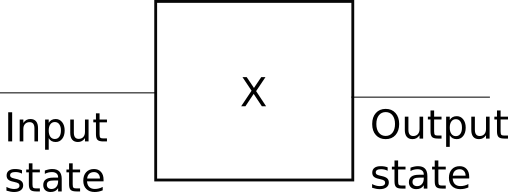
\includegraphics[scale=0.5]{graph/1.png}
\end{figure}
\\
Quantum wire: The qubit is carried along by this Quantum wire until it reaches the X gate, not necessarily means that it carries qubit through space, may represnt a stationary qubit which is simply sitting there, passing through time until the X gate is applied.
\begin{equation*}
\begin{aligned}
	X\ket{0} &= 
\begin{pmatrix}
	0 & 1 \\
	1 & 0 
\end{pmatrix}
\begin{pmatrix}
1 \\
0
\end{pmatrix}
=
\begin{pmatrix}
0 \\
1
\end{pmatrix}
=\ket{1} 
\\
X\ket{1} &= 
\begin{pmatrix}
	0 & 1 \\
	1 & 0 
\end{pmatrix}
\begin{pmatrix}
0 \\
1
\end{pmatrix}
=
\begin{pmatrix}
1 \\
0
\end{pmatrix}
= \ket{0}
\end{aligned}
\end{equation*}
\begin{center}
Quantum NOT gate
\end{center}
\end{example}
\begin{postu}
	The time evolution of the state of a closed quantum system by Schr$\ddot{o}$dinger equation:
\[
i\hbar\frac{\partial \ket{\psi}}{\partial t} = \mathcal{H}\ket{\psi}
\] 
if $\mathcal{H}$ is independent of time
\[
	U(t_{1},t_{2}) = e^{-i\mathcal{H}(t_{2}-t_{1})/\hbar}
\] 
if $\mathcal{H}$ depends on time, we have to do the integration on Hamiltonian
\end{postu}
\begin{postu}[General Measurement]
	Quantum measurements are described by a collection $\{M_{n}\}$ of measurement operators. There are operators acting on the state space of the system being measured. The index m refers to the measurement outcomes that may occur in the experiment. If the state of the quantum system is $\ket{\psi}$ immediately before the measurement then:
\begin{enumerate}
	\item The probability that result m occurs is given by 
		\[
			p(m) = \braket{\psi|M_{m}^{\dagger}M_{m}|\psi}
		\] 
	\item And the state of the system after the measurement is 
		\[
			\frac{M_{m}\ket{\psi}}{\sqrt{\braket{\psi|M_{m}^{\dagger}M_{m}|\psi}}}
		\] 
\end{enumerate}
The measurement operators satisfy the completeness equation $\sum^{}_{m} M^{\dagger}_{m}M_{m}=\mathds{1}$ 
\end{postu}
\begin{example}
\textbf{Measurement of a qubit in the computation basis}
\begin{equation*}
\begin{aligned}
	\ket{\psi} &= \alpha\ket{0}+\beta\ket{1}\\
				  &=	\frac{1}{\sqrt{2}}[(\alpha+\beta)\ket{+}+(\alpha-\beta)\ket{-}] \\
\end{aligned}
\end{equation*}
\begin{equation*}
\begin{aligned}
	M_{0} &= \ket{0}\bra{0}=M_{0}^{\dagger} \\
	M_{1} &= \ket{1}\bra{1}=M_{1}^{\dagger}
\end{aligned}
\end{equation*}
\begin{itemize}
	\item Probability
		\[
			p(0) = \braket{\psi|M_{0}^{\dagger}M_{0}|\psi} = \braket{\psi|M_{0}|\psi} = \abs{\alpha}^{2}
		\] 
		\[
			p(1) = \braket{\psi|M_{1}^{\dagger}M_{1}|\psi} = \braket{\psi|M_{1}|\psi} = \abs{\beta}^{2}
		\] 
	\item Post-Measurement
\[
	\frac{M_{m}\ket{\psi}}{\sqrt{\braket{\psi|M_{m}^{\dagger}M_{m}|\psi}}}=\frac{\alpha}{\sqrt{\abs{\alpha}^{2}}}\ket{0}=\frac{\alpha}{\abs{\alpha}^{2}}\ket{0}=e^{i\theta}\ket{0}
\] 
\end{itemize}
\end{example}
\begin{remark}
\[
\mathcal{O}=
\begin{pmatrix}
	\mathcal{O}_{00} & \mathcal{O}_{01} \\
	\mathcal{O}_{10} & \mathcal{O}_{11} \\
\end{pmatrix}
\ and \ 
\mathcal{O} = \sum^{}_{i,j} \mathcal{O}_{ij}\ket{i}\bra{j}
\] 
\end{remark}
\begin{remark}
Global phase doesn't matter, but relative phase does.
\end{remark}
\newpage
\paragraph{Bloch Shpere representation}%
\ \\
\begin{figure}[!hbt]
\centering
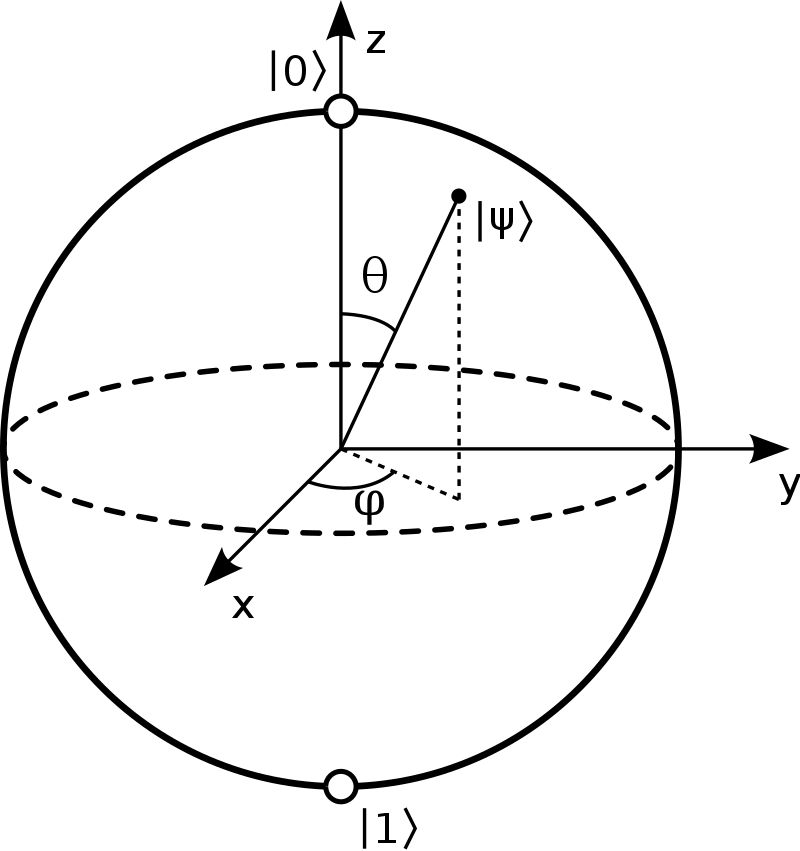
\includegraphics[scale=0.1]{graph/2.png}
\end{figure}
\begin{equation*}
\begin{aligned}
	& \hat{n}=(\sin{\theta}\cos{\phi},\sin{\theta}\sin{\phi},\cos{\phi})\\
	& \ket{+}_{\hat{n}}=\cos{\frac{\theta}{2}}\ket{0}+e^{i\phi}\sin{\frac{\theta}{2}} \ket{1} \\
	& \ket{-}_{\hat{n}}=-\sin{\frac{\theta}{2}}\ket{0}+\cos{\frac{\theta}{2}} e^{i\phi}\ket{1}
\end{aligned}
\end{equation*}
$\ket{+}_{n}$ means the eigenstate of Pauli matrix in $\hat{n}$ direction. That is, $\hat{\sigma} \cdot \hat{n}$. \\
For arbitrary state, the expectation value $\braket{X}^{2}+\braket{Y}^{2}+\braket{Z}^{2}=1$
\begin{remark}
	In Quantum Mechanics, we can not determined all spin component simultaneously since $[S_{i},S_{j}]=i\hbar\epsilon_{ijk}S_{k}$. Hence, in quantum case, we can only calculate the expectation value of three obervables $S_{x},S_{y},S_{z}$.
\end{remark}
\begin{remark}
\\
\[
	\textit{qubit: } \ket{\psi} = \cos{\frac{\theta}{2}}\ket{0}+\sin{\frac{\theta}{2}}e^{i\phi}\ket{0}
\] 
Since $\theta$ and $\phi$ are continuous, it seems that we can carry all information in $\theta$ and $\phi$. However, if we want to extract the probability of $\ket{0}$, we have to prepare "many" pure state. But the precision of the coefficient is related to how many pure state we observe. If we can do measurement infinitely, then we can get exact qunit.  
\end{remark}
\paragraph{Distinguishing Quantum States}%
\ \\
\\
Distinguishibility: a set of states $\ket{\psi_{i}}$, $1 \leq i \leq n$ known to Alice and Bob. Alice choose a state $\ket{\psi_{i}}$ and gives it to Bob, whose task is to identify the index j of the state Alice has given him.
\begin{enumerate}
	\item Suppose $\ket{\psi_{i}}$ are orthonormal $\braket{\psi_{i}|\psi_{j}}=\delta_{ij}$. Define $M_{j}=\ket{\psi_{j}}\bra{\psi_{j}}$. If the state $\ket{\psi_{j}}$ is prepared, then $p(j)=\braket{\psi_{j}|M_{j}^{\dagger}M_{j}|\psi_{j}}=1$ ; $p(i)=\braket{\psi_{i}|M_{j}^{\dagger}M_{j}|\psi_{i}}=0$. 
\begin{remark}
	Since Alice only choose n states, there are some states that are not chosen. Hence, we adjust the completness relation $ \sum^{n}_{i=1} M_{i}^{\dagger}M_{i} + M_{0}^{\dagger}M_{0}=\mathbb{1}$. $M_{0}$ is the rest of the states.
\end{remark}
	\item If the state $\ket{\psi_{i}}$ are not orthonormal then there is no Quantum measurement capable of distinguishing these state. $\braket{\psi_{i}|\psi_{j}}\neq 0$ for $i\neq j$
\end{enumerate}
\begin{postu}[Projective measurement]
A projective measurement is described by an observable, a Hermitian operator $\mathcal{M}$ with spectral decomposition
\[
\mathcal{M}= \sum^{}_{m} m P_{m}
\] 
where $P_{m}=\ket{m}\bra{m}$ is the projector onto the eigenspace of $\mathcal{M}$ with eigenvalue m. \\ \\
The possible outcomes of the measurement correspond to the eigenvalues m and the outcome m occurs with probability
\[
	p(m)=\braket{\psi|P_{m}|\psi}
\] 
The corresponding post-measurement is 
\[
	\frac{P_{m}\ket{\psi}}{\sqrt{\braket{\psi|P_{m}|\psi}}}
\] 
\end{postu}
\begin{example}
\[
S_{z}=
\frac{\hbar}{2}\ket{+}\bra{+} - \frac{\hbar}{2}\ket{-}\bra{-} 
\] 
\end{example}
\begin{remark}
Projective measurement can be usderstood as a special case of general  measurement
\[
	\sum^{}_{m} M^{\dagger}_{m}M_{m}=\mathbb{1}
\] 
From postulate of projective measurement, $M_{m}^{\dagger}=M_{m} (Hermition)$ and $M_{m}M_{m'}=M_{m}\delta_{mm'} (Orthogonal Projector)$  $p(m) = \braket{\psi|M^{\dagger}_{m}M_{m}|\psi}=\braket{\psi|M_{m}|\psi}$ and $\frac{M_{m}\ket{\psi}}{\sqrt{\braket{\psi|M^{\dagger}_{m}M_{m}|\psi}}}=\frac{M_{m}\ket{\psi}}{\sqrt{p(m)}}=\frac{M_{m}\ket{\psi}}{\sqrt{\braket{\psi|M_{m}|\psi}}}$
\end{remark}
\paragraph{The Heisenberg uncertainty principle}%
\label{par:the_heisenberg_uncertainty_principle}
\ \\
\\
Suppose A and B are two Hermitian operators $A^{\dagger}=A, B^{\dagger}=B$. Suppose $\braket{\psi|AB|\psi}=x+iy$ where $x,y \in \mathbb{R}$ 
\[
\braket{\psi|BA|\psi}=\braket{\psi|B^{\dagger}A|\psi}=\braket{\psi|A^{\dagger}B|\psi}^{*}=\braket{\psi|AB|\psi}^{*}
\] 
\[
	\braket{\psi|[A,B]|\psi}=\braket{\psi|AB-BA|\psi}=2iy
\] 
\[
	\braket{\psi|\{A,B\}|\psi}=\braket{\psi|AB+BA|\psi}=2x
\] 
\[
	\abs{\braket{\psi|[A,B]|\psi}}^{2}+\abs{\braket{\psi|\{A,B\}|\psi}}^{2}=4\abs{\braket{\psi|AB|\psi}}^{2}
\] 
By the Cauchy-Schwartz inequality:
\[
\abs{\braket{\psi|AB|\psi}}^{2} \leq \braket{\psi|A^{2}|\psi}\braket{\psi|B^{2}|\psi}
\] 
Hence
\[
	\abs{\braket{\psi|[A,B]|\psi}}^{2}\leq 4\abs{\braket{\psi|AB|\psi}}^{2}\leq 4\braket{\psi|A^{2}|\psi}\braket{\psi|B^{2}|\psi}
\] 
Suppose C and D are two obervables and $A=C-\braket{C}, B=D-\braket{D}$$\Rightarrow [A,B]=[C,D]$
\[
	\abs{\braket{\psi|[C,D]|\psi}}^{2} \leq 4(\Delta C)^{2}(\Delta D)^{2}
\] 
\[
	\frac{1}{2}\abs{\braket{\psi|[C,D]|\psi}}\leq (\Delta C)(\Delta D)
\] 
There is an intrinsic limit to the accureacy of the simultaneous measurement of both C and D if $[C,D]\neq 0.$ \\
The measurement of one observable necessarily disturbs the other if $[C,D]\neq 0$
\paragraph{Positive Operator-valued Measure (POVM) measurement}%
\ \\
\\
\textbf{Positive operator:} A special subclass of Hermitian operators defined as for any vector $\ket{v}, \braket{v|A|v}$ is a real, non-negative numbers.\\
\\
\textbf{Positive definite:} If $\braket{v|A|v}$ is strictly greater than zero for all $\ket{v}\neq 0$\\
\\
\textbf{POVM:} A set of $\{E_{m}\}, \sum^{}_{m} E_{m}=\mathbb{1}, p(m)=\braket{\psi|E_{m}|\psi}$
\begin{remark}
	POVM is a simple consequence of the general measurement. The set of $E_{m}$ is sufficient to determine probabilriy of different outcomes m. The complete set $\{E_{m}\}$ is known as POVM. $E_{m}$ is the POVM element.
\end{remark}
\begin{example}
\begin{equation*}
\begin{aligned}
	\ket{{\psi_{1}}}&=\ket{0}\\
	\ket{\psi_{2}}&=\frac{\ket{0}+\ket{1}}{\sqrt{2}}
\end{aligned}
\end{equation*}
It is impossible for Bob to perform a measurement which distinguishes the states. \\
Consider POVM containing 
\begin{equation*}
\begin{aligned}
	E_{1}&=\frac{\sqrt{2}}{1+\sqrt{2}}\ket{1}\bra{1}\\
	E_{2}&=\frac{\sqrt{2}}{1+\sqrt{2}}\frac{(\ket{0}-\ket{1})(\bra{0}-\ket{1})}{2}\\
	E_{3}&=\mathbb{1}-E_{1}-E_{2}
\end{aligned}
\end{equation*}
If the outcome is $m_{1}$, the state will not be $\ket{\psi_{1}}$ since $\braket{\psi_{1}|E_{1}|\psi_{1}}=0$. The state must be $\ket{\psi_{2}}$.\\
If the outcome is $m_{2}$, the state will not be $\ket{\psi_{2}}$ since $\braket{\psi_{2}|E_{2}|\psi_{2}}=0$. The state must be $\ket{\psi_{1}}$.\\
If the outcome is $m_{3}$, however, we do not sure whether we get $\ket{\psi_{1}}$ or $\ket{\psi_{2}}$. We get no information.
\end{example}
\begin{postu}
The state space of a composite physical system is the tensor product of the state space of the compoment physical system. Moreover, if we have system numbered 1 through n, and the system number i is prepared in the state $\ket{\psi_{i}}$, then the joint state of the total system is
\[
	\ket{\psi_{i}}\otimes\ket{\psi_{2}}\otimes\cdots\ket{\psi_{n}}
\] 
\end{postu}
\begin{example}
\textbf{Two qubit system} \\
Two-qubit state space is $\mathbb{C}^{2}\otimes\mathbb{C}^{2}=\mathbb{C}^{4}$
\begin{equation*}
\begin{aligned}
\ket{0} \\
\ket{1}
\end{aligned}
\otimes
\begin{aligned}
\ket{0} \\
\ket{1}
\end{aligned}
\Rightarrow
\begin{cases}
\ket{0} \otimes \ket{0}  = \ket{0,0} = \ket{0}\ket{0}\\
\ket{0} \otimes \ket{1} \\
\ket{1} \otimes \ket{0} \\
\ket{1} \otimes \ket{1} \\
\end{cases}
\end{equation*}
100 qubits $2^{100}\approx 10^{30}$ memory!! Hilbert space is indeed a big place!
\end{example}
\begin{example}
\[
	(\mathbb{1}\otimes X)\sqrt{0.1}\ket{00}+\sqrt{0.2}\ket{01}+\sqrt{0.3}\ket{10}+\sqrt{0.4}\ket{11}
\] 
\[
= \sqrt{0.1}\ket{01}+\sqrt{0.2}\ket{00}+\sqrt{0.3}\ket{11}+\sqrt{0.4}\ket{10}
\] 
The first operator $\mathbb{1}$ acts on the first qubit space and the second one X acts on the second qubit space.  
\end{example}
\begin{remark}
Through we can compute parallelly, we have to do many measurements to get the information of the amplitute. Thus, we often use interference to left the amplitute of interest and measure it.
\end{remark}
\paragraph{Basic properties of tensor product under $\mathbb{V}\otimes\mathbb{W}$}%
\label{par:basic_properties_of_tensor_product_under_votimesw_}
\\
\begin{enumerate}
	\item $z(\ket{v}\otimes\ket{w}) = z\ket{v}\otimes\ket{w}=\ket{v}\otimes (z\ket{w})\ \ \forall z \in \mathbb{C}$
	\item $\ket{v_{1}}$ and $\ket{v_{2}} \in \mathbb{V}$ and $\ket{w}\in\mathbb{W}$, $(\ket{v_{1}}+\ket{v_{2}})\otimes \ket{w}=\ket{v_{1}}\otimes\ket{w}+\ket{v_{2}}\otimes\ket{w}$
	\item $\ket{v}\otimes(\ket{w_{1}}+\ket{w_{2}})= \ket{v}\otimes\ket{w_{1}}+\ket{v}\otimes\ket{w_{2}}$\\

		Suppose A and B are linear operators on $\mathbb{V}$ and $\mathbb{W}$ respectively.
	\item $(A\otimes B)(\ket{v}\otimes\ket{w})=A\ket{v}\otimes B\ket{w}$ 
	\item $(A\otimes B)( \sum^{}_{i} a_{i}\ket{v_{i}}\otimes\ket{w_{i}})= \sum^{}_{i} a_{i}(A\ket{v_{i}}\otimes B\ket{w_{i}})$ 
	\item
	\[
		A_{m\times n} \otimes B_{p \times q} = \begin{pmatrix} A_{11}B&A_{12}B&\cdots&A_{1n}B\\
		A_{21}B&A_{22}B&\cdots&A_{2n}B\\
		\vdots&\vdots&\ddots&\vdots\\
		A_{m1}B&A_{m2}B&\cdots&A_{mn}B
	\end{pmatrix}_{mp\times nq}
	\] 
\end{enumerate}
\paragraph{Partial measurement}%
\label{par:partial_measurement}\ \\
If the state of a two-qubit system is
\[
\ket{\psi}=\alpha_{0}\ket{00}+\alpha_{1}\ket{01}+\alpha_{2}\ket{10}+\alpha_{3}\ket{11}
\] 
Measure qubit 1 in tis computational basis.
\[
	P_{0}\otimes  \mathbb{1} = \ket{0}\bra{0}\otimes \mathbb{1}
\] 
\[
	P_{1}\otimes \mathbb{1} = \ket{1}\bra{1}\otimes \mathbb{1}
\] 
\begin{equation*}
\begin{aligned}
	P(m=0) &= \braket{\psi|M_{0}^{\dagger}M_{0}|\psi} = \braket{\psi|M_{0}|\psi} = \braket{\psi|P_{0}\otimes \mathbb{1}|\psi } \\
			 &=(\bra{00}\alpha_{0}^{*}+\bra{01}\alpha_{1}^{*}+\bra{10}\alpha_{2}^{*}+\bra{11}\alpha_{3}^{*})(\alpha_{0}\ket{00}+\alpha_{1}\ket{01})\\
			 &= \abs{\alpha_{0}}^{2}+\abs{\alpha_{1}}^{2} \\
	P(m=1) &= \abs{\alpha_{2}}^{2}+\abs{\alpha_{3}}^{2}
\end{aligned}
\end{equation*}
Post-measurement state
\[
	\frac{P_{0}\otimes\mathbb{1}\ket{\psi}}{\sqrt{P(m=0)}} = \frac{\alpha_{0}\ket{00}+\alpha_{1}\ket{01}}{\sqrt{\abs{\alpha_{1}^{2}}+\abs{\alpha_{0}^{2}}}} = \ket{0}\otimes\frac{\alpha_{0}\ket{0}+\alpha_{1}\ket{1}}{\sqrt{\abs{\alpha_{1}^{2}}+\abs{\alpha_{0}^{2}}}} 
\] 
\begin{example}
\[
\psi = \frac{2}{3}\ket{01}+\frac{2}{3}i\ket{10}+\frac{1}{3}\ket{00}
\] 
Measure $1^{st}$ qubit $m_{1}=0$ 
\[
\frac{\frac{2}{3}\ket{01}+\frac{1}{3}\ket{00}}{\sqrt{\frac{2}{3}^{2}+\frac{1}{3}^{2}}} = \frac{2}{\sqrt{5}}\ket{01}+\frac{1}{\sqrt{5}}\ket{00} = \ket{0}\otimes \frac{2\ket{1}+\ket{0}}{\sqrt{5}}
\] 
Measure $2^{nd}$ qubit $m_{2}=0$
\[
\frac{\frac{2}{3}i\ket{10}+\frac{1}{3}\ket{00}}{\sqrt{\frac{2i}{3}^{2}+\frac{1}{3}^{2}}}= \frac{2i\ket{1}+\ket{0}}{\sqrt{5}}\otimes \ket{0}
\] 
Measure $2^{nd}$ qubit $m_{2}=1$
\[
	\frac{\frac{2}{3}\ket{01}}{\sqrt{\frac{2}{3}^{2}}}=\ket{01}=\ket{0}\otimes\ket{1} 
\] 
\end{example}
\paragraph{Quantum entanglement}%
\label{par:quantum_entanglement}
\[
Bell\ state:\ \ket{\psi}=\frac{\ket{00}+\ket{11}}{\sqrt{2}}
\] 
\[
\ket{\psi}\neq \ket{a}\ket{b}\ non-sepearable
\] 
If the state is separable:
\[
	\ket{\psi} = (\alpha\ket{0}+\beta\ket{1})\otimes(\gamma\ket{0}+\delta\ket{1}) = \alpha\gamma\ket{00}+\beta\gamma\ket{10}+\alpha\delta\ket{01}+\beta\delta\ket{11}
\] 
\[
\gamma\beta =  0 \  or \ \alpha\delta=0 \leftrightarrow \alpha\gamma =1 \ and \ \beta\delta = 1
\] 
We describe such state being "entagled state" since they can not be understand in terms of Alice's and Bob's individual system, but rather embody come joint property of the system.\\
\newpage
\textit{Schr$\ddot{o}$dinger(1935): I would not call entangled one but rahter the characteristic trait of quantum mechanics the one thate enforces its entire departure from classical lines of thought.}\\ \\
Suppose the initial system state vector is $\ket{\psi(t)}$, and say, there s a second Quantum system called ancilla system (or the meter) in an initial state $\ket{\phi(t)}$. So the intitial states of the combined system is :
\[
	\ket{\Psi(t)}=\ket{\psi(t)}\otimes\ket{\phi(t)}=\ket{\psi(t)}\ket{\phi(t)}
\] 
Let the two system be coupled together fo a time $T_{1}$
\[
	U(T_1) = e^{-i\mathcal{H}T_{1}/\hbar} \ \ \ \mathcal{H}: total Hamiltonian 
\] 
\begin{equation*}
\begin{aligned}
	\ket{\Psi(t+T_1)}&=U(T_{1})\ket{\psi(t)}\ket{\phi(t)}\\
						  &= \sum^{}_{m} \beta_{m}(t)\ket{\psi_{m}(t)}\ket{\phi_{m}} 
\end{aligned}
\end{equation*}
\[
\ \ \ket{\phi_{m}}\ is\ the\ orthonomal\  basis,\ but\ \ket{\psi_{m}(t)}\ may\ not\ orthogonal. 
\] 
Now let the meter be measured projectively over a small time interval $T_{2}$ and the outcome is m, the post measurement state is 
\[
	\ket{\Psi_{m}(t+T_{1}+T_{2})} = \frac{[\mathbb{1}\otimes \ket{\phi_{m}}\bra{\phi_{m}}]U(T_{1})\ket{\psi(t)}\ket{\phi(t)}}{\sqrt{P_{m}(T_{2})}}=\frac{M_{m}}{\sqrt{P_{m}}}\ket{\phi_{m}}\ket{\psi(t)}
\] 
\begin{equation*}
\begin{aligned}
	P_{m}(T_{2}) &= \braket{\Psi(t+T_{1})|P_{m}|\Psi(t+T_{1})} \\
					 &= \bra{\phi(t)}\bra{\psi(t)}U^{\dagger}(T_{1})[\mathbb{1}\otimes \ket{\phi_{m}}\bra{\phi_{m}}]U(T_{1})\ket{\psi(t)}\ket{\phi(t)}\\
					 &= \braket{\psi(t)|M_{m}^{\dagger}M_{m}|\psi(t)}\ \\ 
\end{aligned}
\end{equation*}
\[
	 \forall M_{m}=\braket{\phi_{m}|U(T_{1})|\phi(t)}\ \textit{acting on the system Hilbert space only }
\] 
The completeness condition:
\begin{equation*}
\begin{aligned}
	\sum^{}_{m} M_{m}^{\dagger}M_{m} &= \sum^{}_{m} \braket{\phi(t)|U^{\dagger}(T_{1})|\phi_{m}}\braket{\phi_{m}|U(T_{1})|\phi(t)}\\
												&=\braket{\phi(t)|U^{\dagger}(T_{1})U(T_{1})|\phi(t)} = \mathbb{1}
\end{aligned}
\end{equation*}
\paragraph{EPR paradox and Bell's inequality}%
\label{par:epr_paradox_and_bell_s_inequality} \ \\ 
\begin{itemize}
	\item Perhaps, the most spectacular and counter-intuitive manifestation of quantum mechanics is the phenonmenon of entanglement observed in composite quantum system. 
	\item According to quantum mechanics, and unobserved particle do not posses physical properties thate exist independent of observation (reality assumption). Rather, such physical arise as a consequence of measurement performed upon the system.
	\item In early days of the development of quantum mechanics, many physicists rejected this view of Nature. The most prominent objector was Albert Einstein.
	\item 1935, Albert Einstein, Nathan Rosen, Boris Podolsky proposed a thought experiment which they believed demonstrated that QM is not a complete theory of Nature $\Rightarrow$ QM leads to a contradiction, provided that we accept the following two seemingly natural assumptions (that Nature ought to obey) \\
		\textbf{(1) Reality principle:}  If we can predict with certainty the value of a physical quantity, then this value has physical reality, independent of observations. e.g. thennis ball, moon, color of a chalk \\
		\textbf{(2) Locality principle:} If two system are causally disconnected, the result of any measurement performed one a system cannot influence the result of a measurement performed the second system.  \\ \\
		\underline{\textbf{Theory of relativity:} } two events taking place at space-time coordinates $(x_{1},t_{1}), (x_{2},t_{2})$ respectively. The two events are disconnected if $(\Delta x)^{2} > (c\Delta t)^{2}$ (Space-like events). That is , physical influence cannot propagate fasten than light.
	\item 1964, John Bell formulated inequality assuming the principle of realism and locality. Since it is possible to \textbf{devise situations} in which QM predicts a violation of these inequalities, any experimental observation of such a violation excludes the possibility of a local and realistic description of natural phenomena.
\begin{remark}
It turns out that Nature experimentally invalidates EPR's points of view, while agreeing with QM. To device Bell's inequality, we should forget about QM for a moment, and use the classical common sense notion of how the world works, the sort of notion EPR thought Nature ought to obey.
\end{remark}
	\item The thought experiment:
\begin{figure}[h]
	\centering
	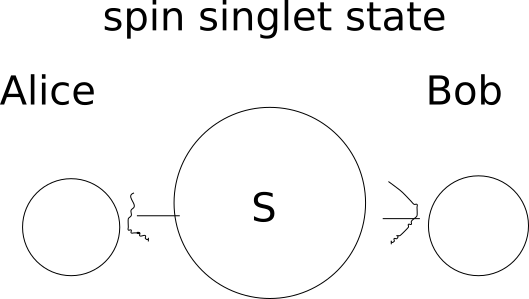
\includegraphics[scale = 0.3]{graph/3.png}
\end{figure}
\begin{enumerate}
	\item A source  that is capable of repeating the experimental procedure to prepare two particle.
	\item Once tha particles are prepared, one particle is sent to A(lice) and the other to B(ob).
	\item The timing of the experiment is arranged so that Alice and Bob do their measurements at the same time (or in a causally disconnected manner). 
	\item Alice and Bob can measure the polarization along 3 different axes a,b,c.
\end{enumerate}
According to the reality principle, we may assign well defined values to the spin components along the three axes. That is, we assume that these values have physical reality independent of our observation. The result of the measurement of Alice and Bob are perfectly anti-correlated.\\
\\
\textbf{Classical intuitive example:} two balls (one black, one white), a pair of gloves (one left-handed, one right-handed)
\begin{equation*}
\begin{aligned}
	Alice &&& Bob \\
	\downarrow &&& \downarrow \\ 
	white &&& black \\
	(L) &&& (R) \\
\end{aligned}
\end{equation*}
\begin{center}
\textit{\textbf{Locality and Reality}}
\end{center}
The result are mutually exclusive groups:
\begin{center}
\begin{tabular}{|c|c|c|}
	\hline
	Population & Alice's particle & Bob's particle \\ 
	\hline 
	$N_{1}$ & $(a_{+},b_{+},c_{+})$ & $(a_{-},b_{-},c_{-})$ \\
	\hline 
	$N_{2}$ & $(a_{+},b_{+},c_{-})$ & $(a_{-},b_{-},c_{+})$ \\
	\hline 
	$N_{3}$ & $(a_{+},b_{-},c_{+})$ & $(a_{-},b_{+},c_{-})$ \\
	\hline 
	$N_{4}$ & $(a_{+},b_{-},c_{-})$ & $(a_{-},b_{+},c_{+})$ \\
	\hline 
	$N_{5}$ & $(a_{-},b_{+},c_{+})$ & $(a_{+},b_{-},c_{-})$ \\
	\hline 
	$N_{6}$ & $(a_{-},b_{+},c_{-})$ & $(a_{+},b_{-},c_{+})$ \\
	\hline 
	$N_{7}$ & $(a_{-},b_{-},c_{+})$ & $(a_{+},b_{+},c_{-})$ \\
	\hline 
	$N_{8}$ & $(a_{-},b_{-},c_{-})$ & $(a_{+},b_{+},c_{+})$ \\
	\hline
\end{tabular}
\end{center}
Let $P(a_{+},b_{+})$ denote the probability that Alice obtains $\sigma^{A}_{a}:+1$ and Bob obtains $\sigma^{B}_{b}:+1$
\[
	P(a_{+},b_{+}) = \frac{N_{3}+N_{4}}{N} \ \ \ P(a_{+},c_{+}) = \frac{N_{2}+N_{3}}{N} \ \ \ P(c_{+},b_{+}) = \frac{N_{3}+N_{7}}{N} 
\] 
\begin{equation*}
\begin{aligned}
	& N_{3}+N_{4} \leq (N_{2}+N_{4}) + (N_{3}+N_{7}) \\ 
	\Rightarrow\ & P(a_{+},b_{+}) \leq P(a_{+},c_{+}) + P(c_{+},b_{+}) \textit{\ \ (Bell's inequality)}
\end{aligned}
\end{equation*}
\textbf{Reality:} We can establish the above table. \\ \\
\textbf{Locality:}
If a pair belongs to group 1, and Alice's choose to measure $\sigma^{A}_{a}$, then she will certainly obtain outcome +1, i.e. $a_{+}$, independently of the fact that Bob may choose to perform a measurement along the axes a,b or c. \\
\begin{center}
\textit{\textbf{Quantum Theory}}
\end{center}
The state of one particle depends unpon the nature of the observable measured on the other particle.
\[
	\ket{\psi} = \frac{1}{\sqrt{2}}(\ket{01}-\ket{10}) = \frac{1}{\sqrt{2}}(\ket{+}\ket{-}-\ket{-}\ket{+})  = \frac{1}{\sqrt{2}}(\ket{+}_{n}\ket{-}_{n}-\ket{-}_{n}\ket{+}_{n}) 
\] 
If Alice finds $\sigma^{A}_{a}:+1$, then the state of Bob's particle collapses to the eigenstate of $\ket{-}_{a}$ $\Rightarrow$ $\sigma^{B}_{b}$ with probability $\braket{\psi|P_{m}|\psi} = _{a}\braket{-|+}_{b} _{b}\braket{+|-}_{a}=\sin^{2}{\frac{\theta_{ab}}{2}}\ \Rightarrow\ P(a_{+},b_{+})=\frac{1}{2}\sin^{2}{\frac{\theta_{ab}}{2}}$ 
\[
	\sin^{2}{\frac{\theta_{ab}}{2}} \leq \sin^{2}{\frac{\theta_{ac}}{2}}+ \sin^{2}{\frac{\theta_{cb}}{2}}\ \ \textit{( Substite in Bell's inequality)}
\] 
If we choose $\theta_{ab} = 2\theta, \theta_{ac}=\theta_{cb}= \theta$, then the inequality becomes $\sin^{2}{\theta}\leq 2\sin^{2}{\frac{\theta}{2}}$. If $\theta = 60^{o} \Rightarrow \left(\frac{\sqrt{3}}{2}\right)^{2}\leq 2 \left(\frac{1}{2}\right)^{2}\Rightarrow \frac{3}{4}\leq \frac{2}{4}\ !!!!$ \textbf{The Quantum Mechanics will violate Bell's inequatlity.}\\
	\item 1968, \textbf{CHSH(Clauser, Horne, Shimony and Holt) inequality.} (Example of a larger set of Bell's inequalities) \\
\begin{figure}[h]
	\centering
	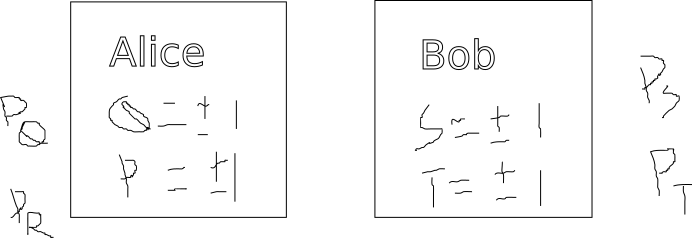
\includegraphics[scale = 0.3]{graph/4.png}
\end{figure}
\\
They do not decide which property she or he will measure. 
\begin{center}
\textit{\textbf{Reality and Locality}}
\end{center}
\textbf{Reality:} physical properties of $P_{Q},P_{R},P_{S},P_{T}$ have definite values Q,R,S,T which exist independent of observation. \\
\\
\textbf{Locality:} Timing of measurement $\Rightarrow$ Causally disconnected! The measurement which Alice performed cannot disturb the result of Bob's measurement (or vice versa). 
\\ \\ 
\[
	QS+RS+RT-QT = (Q+R)S+(R-Q)T = \pm 2
\] 
\[
	(Suppose\ R,Q = \pm 1.\ Thus,\ (R+Q)S=0\ or\ (R-Q)T=0)
\] 
\\
Emsemble average:\ (The curly words mean operator)
\[
	E(\mathcal{QS+RS+RT-QT}) = \sum^{}_{} p(Q,R,S,T)(QS+RS+RT-QT) \leq \sum^{}_{} p(Q,R,S,T)\cdot2 = 2
\] 
\begin{center}
\textit{\textbf{Quantum Theory}}
\end{center}
\[
	E(\mathcal{QS+RS+RT-QT}) = \braket{\psi|\mathcal{QS+RS+RT-QT}|\psi} = \braket{\mathcal{QS}} + \braket{\mathcal{RS}} +\braket{\mathcal{RT}} - \braket{\mathcal{QT}} 
\] 
\begin{example}
\[
	\ket{\psi}=\frac{1}{\sqrt{2}}(\ket{01}-\ket{10})
\] 
\[
Q=Z_{1}\ \ R=X_{1}\ \  S= \frac{-Z_{2}-X_{2}}{\sqrt{2}}\ \ T= \frac{Z_{2}-X_{2}}{\sqrt{2}}
\] 
\[
\braket{\mathcal{QS}} + \braket{\mathcal{RS}}+ \braket{\mathcal{RT}} -\braket{\mathcal{QT}} = 2\sqrt{2} > 2 !!\textit{\textbf{ The Quantum Theory violates Bell's inequality.}}
\] 
\end{example}
	\item 1981. \textit{Violation of CHSH inequality and an excellent agreement with QM}
\begin{itemize}
	\item Photon detection efficiency $\eta \approx 0.05 ~ 0.33$
	\item Seperation between trapped ions $d\approx 1m$
\end{itemize}
	A loophole-free experiment will require.
\begin{itemize}
	\item Spacelike separation between Alice's and Bob's measurements (locality loophole)
	\item Sufficient large number of detections of the prepared particles (detection loophole)
\end{itemize}
\begin{enumerate}
	\item B.Hensen et al., Nature 528, 682 (2015)
	\item M.Giustina et al. Physical Review Letters 115, 250401 (2015)
	\item L.K.Shalin et al. Physical Review Letters 115, 250402 (2015)
\end{enumerate}
	\item 1969, The CHSH Game  \\
		\\
		The game itself does not involved quantum mechanics, but quantum mechanics can help us win it. Alice and Bob are placed in separate rooms and are each given a challenge bit (x and y, respectively). The challenge bits are chosen uniformly at random, and indpendently of each other. Then Alice sends an answer bit $a$ back to the refree, and Bob sends back an answer bit $b$. Alice and Bob win the game iff
\[
	a+b = xy \mod2
\] 
So if either x or y is 0: a and b should be equal. But if x=y=1: a and b should be different. \\
\\
Alice and Bob are allowed to agree on a strategy in advance and to share random bits.
\begin{center}
\textbf{Classical Strategy}
\end{center}
The classical strategy to maximize winning probability simply that Alice and Bob always send the refree a=b=0 regardless of what x and y are. In this case, Alice and Bob win $75\%$ of the time, losing only if x and y are both 1. The Bell's inequality, in this framework, is just the slightly-boring statement that the maximum classical win probability in the CHSH game is $75\%$. 
\begin{center}
\textbf{Quantum Strategy}
\end{center}
If Alice and Bob had pre-shared Bell pair $\frac{\ket{00}+\ket{11}}{\sqrt{2}}=\frac{\ket{++}+\ket{--}}{\sqrt{2}}$, then there is a better strategy
\begin{figure}[h]
	\centering
	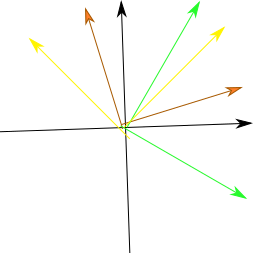
\includegraphics[scale=0.5]{graph/5.png}
\end{figure}
\[
	\ket{\frac{\pi}{8}}=\cos{(\frac{\pi}{8})}\ket{0}+\sin{(\frac{\pi}{8})}\ket{0}
\] 
\[
	\ket{+} = \cos{(\frac{\pi}{4})}\ket{0}+\sin{(\frac{\pi}{4})}\ket{1}
\] 
\[
	\ket{-\frac{\pi}{8}}=\cos{(-\frac{\pi}{8})}\ket{0}+\sin{(-\frac{\pi}{8})}\ket{0}
\] 
The strategy:\\ \\
If x = 0, Alice measure in $\{\ket{0},\ket{1}\}$ and if x = 1, Alice measure in $\{\ket{+},\ket{-}\}$.  She sets a to 0 if she measures $\ket{0}$ and $\ket{+}$ and 1 if she measures $\ket{1}$ or $\ket{-}$ \\
If y = 0, Bob measure in $\{\ket{\frac{\pi}{8}},\ket{\frac{\pi}{8}+\frac{\pi}{2}}\}$ and if y = 1, Bob measure in $\{\ket{-\frac{\pi}{8}},\ket{-\frac{\pi}{8}+\frac{\pi}{2}}\}$. He sets b to 0 if he measures $\ket{\frac{\pi}{8}}$ or $\ket{-\frac{\pi}{8}}$ and 1 if otherwise.\\
\\
\textbf{Let's consider the case where Alice gets x=0 and measure $\ket{0}$.}\\ \\ She will output $a=0$, and she and Bob will win iff Bob outputs  $b=0$. Given that Alice measured her qubit already, Bob's qubit collapsed to the  $\ket{0}$ state. First suppose y = 0, Then Bob measures the state $\ket{0}$ in the  $\ket{\frac{\pi}{8}}$ basis. He outputs $b=0$ if he measure $\ket{\frac{\pi}{8}}$. Thus, the probability that Bob output 0 in this case is $|\braket{\frac{\pi}{8}|0}|^{2}=\cos^{2}{\frac{\pi}{8}}\approx 85\%$. For y = 1, Bob measure in $\ket{0}$ in $\ket{-\frac{\pi}{8}}$ basis. The probabiltiy that Bob output 0 in this case $\approx 85\%$ \\ \\
\textbf{Consider the case where Alice gets x=1 and Bob gets y=1. Alice measure $\ket{-}$} \\ \\ She will output a = 1, and she and Bob will win iff Bob outputs b = 0. Given that Alice measured her qubit already, Bob's qubit collapsed to the  $\ket{-}$ state. Bob measure in $\ket{-}$ in $\ket{-\frac{\pi}{8}}$ basis. The probabiltiy that Bob output 0 in this case is still $|\braket{-|-\frac{\pi}{8}}|^{2}$ $\approx 85\%$ \\
\item \textbf{Entanglement EPR steering and Bell's nonlocality}
\begin{figure}[h]
\centering
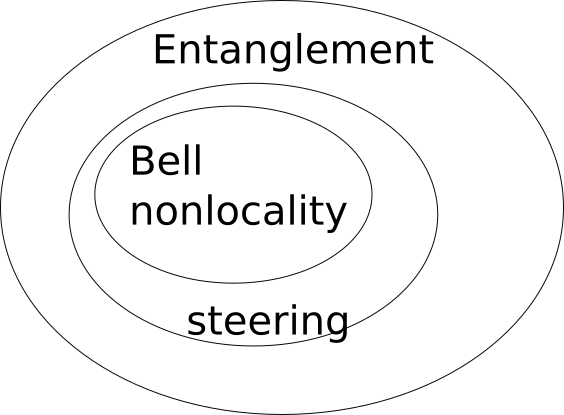
\includegraphics[scale=0.4]{graph/6.png}
\end{figure}
\begin{itemize}
	\item Entanglement: non-seperable to product state
	\item Bell's nonlocality: violation of Bell's inequality
	\item Steering: Manipulate the other state.
\end{itemize}
\item \textbf{1982, No-cloning theorem }
\begin{itemize}
	\item Quantum mechanics does not allow the copying of arbitrary quantum state or no arbitrary copying by unitary transformation. \\
	\item It is not possible to make a copy of an arbitrary unknown quantum state.
\end{itemize}
\begin{proof}
Suppose we have a quantum machine $data\ slot\ \ket{\psi}$ and $target\ slot\ \ket{s}$
\[
\ket{\psi}\otimes\ket{s}\rightarrow U(\ket{\psi}\otimes\ket{s})=\ket{\psi}\otimes\ket{\psi}
\] 
Proof 1
\[
	U(\ket{\psi_{1}}\otimes\ket{\psi_{1}})=\ket{\psi_{1}}\otimes\ket{\psi_{1}}
\] 
\[
	U(\ket{\psi_{2}}\otimes\ket{\psi_{1}})=\ket{\psi_{2}}\otimes\ket{\psi_{2}}
\] 
\[
	U((\ket{\psi_{2}}+\ket{\psi_{1}})\otimes\ket{\psi_{1}})=(\ket{\psi_{2}}+\ket{\psi_{1}})\otimes (\ket{\psi_{2}}+\ket{\psi_{1}})
\] 
But
\[
	U((\ket{\psi_{2}}+\ket{\psi_{1}})\otimes\ket{\psi_{1}})=U(\ket{\psi_{1}}\otimes\ket{\psi_{1}}) + U(\ket{\psi_{2}}\otimes\ket{\psi_{1}}) = \ket{\psi_{1}}\otimes\ket{\psi_{1}}+\ket{\psi_{2}}\otimes\ket{\psi_{2}}\Leftrightarrow
\] 
Proof 2
\[
	U(\ket{\psi}\otimes\ket{s}) = \ket{\psi}\otimes \ket{\psi}
\] 
\[
	U(\ket{\phi}\otimes\ket{s}) = \ket{\phi}\otimes \ket{\phi}
\] 
Take the inner product
\[
\braket{\psi|\phi}\braket{\psi|\phi}=\bra{\psi}\otimes\bra{s}U^{\dagger}U\ket{\phi}\otimes\ket{s} = \braket{\psi|\phi}\braket{s|s} = \braket{\psi|\phi}
\] 
So a cloning device can only clone states which are orthogonal to one another and therefore a general quantum cloning device is not possible. Hence, a potential quantum machine cannot clone both $\ket{\psi}=\ket{0}$ and $\ket{\phi}=\frac{\ket{0}+\ket{1}}{\sqrt{2}}$ since these states are not orthogonal.
\end{proof}
\end{itemize}
\paragraph{Quantum Circuit Model}%
\label{par:quantum_circuit_model}  \ \\
\begin{equation*}
\begin{aligned}
	&\textit{Pauli gate}\ \ \ 
	\Qcircuit @C=1.4em @R=0.7em{
		& \gate{X} & \qw
	}
	\ \ \ X=\begin{pmatrix} 0&1\\1&0 \end{pmatrix}\  \ \
	\Qcircuit @C=1.4em @R=0.7em{
		& \gate{Y} & \qw		
	}
	\ \ \ Y = \begin{pmatrix} 0&-i\\i&0 \end{pmatrix}\ \ \ 
	\Qcircuit @C=1.4em @R=0.7em{
		& \gate{Z} & \qw 
	}
	\ \ \ Z = \begin{pmatrix} 1&0\\0&-1 \end{pmatrix} \\
	&\textit{Hadamard gate} \ \ \ 
	\Qcircuit @C=1.4em @R=0.7em{
		& \gate{H} & \qw
	}
	\ \ \ H=\frac{1}{\sqrt{2}}\begin{pmatrix} 1&1\\1&-1 \end{pmatrix} =\frac{1}{\sqrt{2}}(Z+X)\ \ \ H\ket{0}=\frac{1}{\sqrt{2}}(\ket{0}+\ket{1})\ \ \ H\ket{1}=\frac{1}{\sqrt{2}}(\ket{0}-\ket{1})\\
	&\textit{Phase gate}\ \ \ 
	\Qcircuit @C=1.4em @R=0.7em{
		& \gate{S} & \qw
	}
	\ \ \ S=\begin{pmatrix} 1&0\\0&i \end{pmatrix}\ \ \   
	\textit{$\frac{\pi}{8}$ gate} \ \ \
	\Qcircuit @C=1.4em @R=0.7em{
		& \gate{T} & \qw
	}
	\ \ \ T=\begin{pmatrix} 1&0\\0&e^{i\frac{\pi}{4}} \end{pmatrix} \\
\end{aligned}
\end{equation*}
\[
	 X^{2}=Y^{2}=Z^{2}=H^{2}=I \ \ \ S^{2}=Z\ \ \ T^{2}=S
\] 
\textit{Rotation operator}
\[
	R_{\hat{n}}(\theta) = e^{-i\frac{\theta}{2}(\hat{n}\cdot \sigma )} = \cos{(\frac{\theta}{2})}I+\sin{(\frac{\theta}{2})}(\hat{n}\cdot \sigma)
\] 
\textit{Unitary single-qubit gate (Rotate qubit on Bloch's sphere)} 
\[
	\Qcircuit @C=1.4em @R=0.7em{
		& \gate{U} & \qw
	}\ \ \ 
	U=e^{i\delta}R_{z}(\alpha)R_{y}(\gamma)R_{z}(\beta) = \begin{pmatrix} e^{i(\delta-\frac{\alpha}{2}-\frac{\beta}{2})}\cos{(\frac{\gamma}{2})}&-e^{i(\delta-\frac{\alpha}{2}+\frac{\beta}{2})}\sin{(\frac{\gamma}{2})}\\e^{i(\delta+\frac{\alpha}{2}-\frac{\beta}{2})}\sin{(\frac{\gamma}{2})}&e^{i(\delta+\frac{\alpha}{2}+\frac{\beta}{2})}\cos{(\frac{\gamma}{2})} \end{pmatrix} 
\] 
\textit{Transformation of gate}
\begin{equation*}
\begin{aligned}
	&\Qcircuit @C=1.4em @R=0.7em{
		& \gate{H} & \gate{X} & \gate{H} & \qw 
	} \ \ \
	HXH=\frac{1}{\sqrt{2}}(X+Z) X \frac{1}{\sqrt{2}}(X+Z) = \frac{1}{2}(X+Z+Z+ZXZ)=Z \\
	&\Qcircuit @C=1.4em @R=0.7em{
	& \gate{H} & \gate{Y} & \gate{H} & \qw
	} \ \ \ 
	HYH = \frac{1}{\sqrt{2}}(X+Z)Y\frac{1}{\sqrt{2}}(X+Z) = \frac{1}{2}(XYX + ZYX + XYZ + ZYZ) = -Y \\
	&\Qcircuit @C=1.4em @R=0.7em{
		& \gate{H} & \gate{Z} & \gate{H} & \qw 
	} \ \ \
	HZH=\frac{1}{\sqrt{2}}(X+Z) Z \frac{1}{\sqrt{2}}(X+Z) = \frac{1}{2}(XZX+X+Z+X)=X \\
\end{aligned}
\end{equation*}
It can be verfied from commuation and anti-commutaion relation
\[
	\{\sigma_{i},\sigma_{j}\} = 2\delta_{ij}I \ \ \ [\sigma_{i},\sigma_{j}] = 2i\epsilon_{ijk}\sigma_{k}
\] 
\textbf{Two qubit gates} \\ \\
\textit{\textbf{CNOT gate (controlled-not)}}
\[
\Qcircuit @C=1.4em @R=0.7em{
	& \multigate{1}{CNOT} & \qw \\
	& \ghost{CNOT} & \qw
}
\] 
\\
\[
\Qcircuit @C=1.4em @R=0.0em @!R {
	\lstick{Contorl\ bit}& \ctrl{2} & \qw &&& \ctrl{2} & \qw \\
	&&&\push{\rule{0em}{0.0em}=\rule{0em}{0.0em}}&& \\
	\lstick{Target\ bit}& \gate{X} & \qw &&& \targ & \qw\\
}
\] 
\\
\begin{equation*}
\begin{aligned}
\ket{00} \rightarrow \ket{00} \\
\ket{01} \rightarrow \ket{01} \\
\ket{10} \rightarrow \ket{11} \\
\ket{11} \rightarrow \ket{10} \\
\end{aligned}
\ \ \ \ CNOT=\begin{pmatrix} 1&0&0&0\\0&1&0&0\\0&0&0&1\\0&0&1&0 \end{pmatrix} 
\end{equation*}
\\
\[
\Qcircuit @C=1.4em @R=0.7em{
	\lstick{\ket{\psi}} & \ctrl{1} & \rstick{\ket{\psi}} \qw \\
	\lstick{\ket{\phi}} & \targ & \rstick{\ket{(\psi+\phi) mod 2}} \qw 
}
\] 
\\
Thus, CNOT gate can reproduce $\ket{0}$ and $\ket{1}$
\[
\Qcircuit @C=1.4em @R=0.7em{
	\lstick{\ket{\psi}} & \ctrl{1} & \rstick{\ket{\psi}} \qw \\
	\lstick{\ket{0}} & \targ & \rstick{\ket{\psi}} \qw  
}
\] 
\\
CNOT gate combined with Hadamard gate can transform basis state into Bell state
\[
\Qcircuit @C=1.4em @R=0.7em{
	\lstick{\ket{0}} & \gate{H} & \ctrl{1} & \rstick{\frac{1}{\sqrt{2}}(\ket{0}+\ket{1})} \qw \\
	\lstick{\ket{0}} & \qw & \targ & \rstick{\ket{\psi}} \qw  
}
\] 
Thus, we can not determined $\ket{\psi}$. $\ket{\psi}$ is entangled with control bit now
\[
	\ket{Control}\otimes \ket{Target} = \frac{1}{\sqrt{2}}(\ket{00}+\ket{11})
\] 
In general, if one of input state is superposed, the output will entangle. It can be computed by matrix.
\[
	\Qcircuit @C=1.4em @R=0.7em{
		\lstick{\alpha\ket{0}+\beta\ket{1}} & \ctrl{1} & \rstick{?} \qw \\
		\lstick{\gamma\ket{0}+r\ket{1}} & \targ & \rstick{?} \qw \\ 
	}
\] 
\\
\textit{\textbf{CZ gate (controlled-Z)}}
\[
\Qcircuit @C=1.4em @R=0.0em @!R { \lstick{Contorl\ bit}& \ctrl{2} & \qw &&& \gate{Z}   & \qw \\
	&&&\push{\rule{0em}{0.0em}=\rule{0em}{0.0em}}&& \\
	\lstick{Target\ bit}& \gate{Z} & \qw &&& \ctrl{-2}  & \qw\\
}
\] 
\begin{equation*}
\begin{aligned}
	\ket{00} \rightarrow &\ket{00} \\
\ket{01} \rightarrow &\ket{01} \\
\ket{10} \rightarrow &\ket{10} \\
\ket{11} \rightarrow &-\ket{11} \\
\end{aligned}
\ \ \ \ CZ=\begin{pmatrix} 1&0&0&0\\0&1&0&0\\0&0&1&0\\0&0&0&-1 \end{pmatrix} 
\end{equation*}
\\
\\
\textit{\textbf{Relation between CNOT and CZ gate}}
\[
\Qcircuit @C=1.4em @R=0.0em @!R { 
	\lstick{Contorl\ bit}& \ctrl{2} & \qw &&& \qw & \ctrl{2} &\qw    & \qw \\
								&&&\push{\rule{0em}{0.0em}=\rule{0em}{0.0em}}&&&& \\
	\lstick{Target\ bit}& \gate{Z} & \qw &&& \gate{H} & \targ & \gate{H} & \qw\\
}
\] 
\[
\Qcircuit @C=1.4em @R=0.0em @!R { 
	\lstick{Contorl\ bit}& \ctrl{2} & \qw &&& \qw & \ctrl{2} &\qw    & \qw \\
								&&&\push{\rule{0em}{0.0em}=\rule{0em}{0.0em}}&&&& \\
	\lstick{Target\ bit}& \targ  & \qw &&& \gate{H} & \gate{Z}  & \gate{H} & \qw\\
}
\] 
\\
\textbf{Classical computation} \\
\\
AND, OR, NAND, XOR, NOT \\
\begin{figure}[h]
\centering
	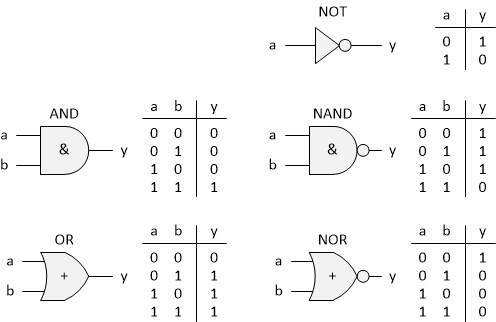
\includegraphics[scale = 0.5]{graph/10.png}
\end{figure}
\\
Universal gate: NAND gate can be used to simulate the AND, OR, XOR and NOT gate, provided wires ancilla bits and Fanout are available.\\
\begin{figure}[h]
\centering
	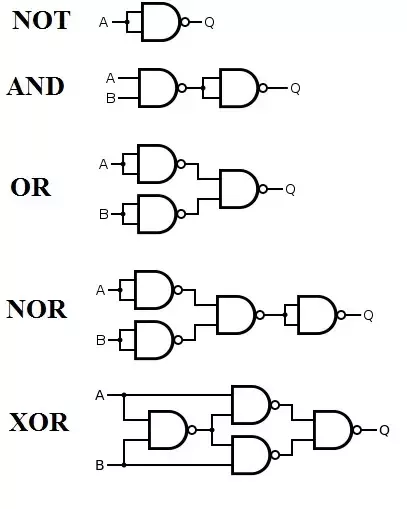
\includegraphics[scale = 0.5]{graph/11.png}
\end{figure}
\newpage
\ \\
\textit{1961, Rolf Landauer: Only process in a computation which are irreversible are those which erase information. Any irreversible operation in a computation is necessarily accompanied by heat dissipation into the environment.} \\
\\
Erasing one bit $\Rightarrow$ reducing the number of state by a factor of 2 $\Rightarrow$ reduce the entropy of the computer by $k_{B}\ln{2}$ $\Rightarrow$ the entropy of the entire universe cannot decrease $\Delta S_{computer}=-k_{B}\ln{2}$ $\Rightarrow$ $\Delta S_{rest}\geq k_{B}\ln{2}$
\[
	\Delta Q_{rest}=T\Delta S_{rest} = k_{B}T\ln{2}
\] 
\textit{1973, Chales Bennett, main trick to computer using only reversible circuit elements by embedding the gate in a larger reversible gate, possibly making use of some extra ancilla bits.} \\
\\
\textit{1982, Ed Fredkin\& Tom Toffoli showed independently the way to bulid reversible computation. By avoiding to erase information, one creates and also must carry along a signigicant amount of redundancy.} \\
\[
\Qcircuit @C=1.4em @R=0.7em{
	& \mbox{\textbf{Toffoli gate}} \\
	& \ctrl{1} & \qw \\
	& \ctrl{1} & \qw \\
	& \targ    & \qw \\
}
\] 
\\
The information processing by any classical NAND logical gate can be replaced by a Toffoli gate and the ability to prepared and ancilla bit. \textbf{Toffoli gate is universal for classical computation}. \\
\[
\Qcircuit @C=1.4em @R=0.7em{
	& \mbox{Toffoli}\\
	\\
	\lstick{a} & \ctrl{1} & \rstick{a} \qw \\
	\lstick{b} & \ctrl{1} & \rstick{b} \qw \\
	\lstick{c} & \targ    & \rstick{c\oplus ab} \qw \\
} \qquad \qquad \qquad 
\Qcircuit @C=1.4em @R=0.7em{
	& \mbox{NAND} \\
	\\
	\lstick{a} & \ctrl{1} & \rstick{a} \qw & \rstick{\ \ redundancy} \\
	\lstick{b} & \ctrl{1} & \rstick{b} \qw & \rstick{\ \ (garbage\ bit)} \\
	\lstick{1} & \targ    & \rstick{1\oplus ab=NAND(a,b)} \qw & \gategroup{3}{3}{4}{4}{.7em}{--} \\
} \qquad \qquad \qquad  \qquad \qquad  \qquad 
\Qcircuit @C=1.4em @R=0.7em{
	& \mbox{Fanout} \\
	\\
	\lstick{1} & \ctrl{1} & \rstick{1} \qw \\
	\lstick{a} & \ctrl{1} & \rstick{a} \qw \\
	\lstick{0} & \targ    & \rstick{0\oplus a = a} \qw \\
} 
\] 
\\
\\
\textbf{Universal quantum gates}
\begin{enumerate}
	\item Single-qubit gates (arbitrary rotations two orthogonal axes) and CNOT gates (arbitrary entangling gate)
	\item A discrete set of universal operation Hadomard gate, $\frac{\pi}{8}$ gate and CNOT gate. H \& $\frac{\pi}{8}$ gates can be used to approximate any single qubit unitary operation to arbitrary accuracy. (+ phase gate S: Fault-tolerant gate set. Quantum state is much more fragile than classical memory) 
\end{enumerate}
Fault-tolerant QC: In principle, an arbitrarily long QC can be performed reliably provided that the average probability of error per gate is less than a certain critical value (the accuracy/error threshold, which depending on the choice of error correction code (ECC)) \\ \\
\textbf{Two qubit gate decomposition} \\
\[
\Qcircuit @C=1.4em @R=0.7em{
	& \ctrl{2} &\qw && &\qw&\ctrl{2}&\qw&\ctrl{2}&\gate{\begin{pmatrix} 1&0\\0&e^{i\delta} \end{pmatrix} } & \qw \\ 
	& & &=& &&&&& \\ 
	& \gate{U}   &\qw && &\gate{C} &\targ&\gate{B} &\targ&\gate{A} & \qw \\ 
}
\] 
\\
\[
\forall\ \ ABC = I \textit{\ and \ } U=e^{i\delta}AXBXC
\] 
For single qubit state
\[
	U = e^{i\delta}R_{z}(\alpha)R_{y}(\gamma)R_{z}(\beta)
\] 
Let
\[
	A = R_{z}(\alpha)R_{y}(\frac{\gamma}{2}) \ \ \ B=R_{y}(-\frac{\gamma}{2})R_{z}(-\frac{\alpha+\beta}{2})\ \ \ C=R_{z}(\frac{\beta-\alpha}{2})
\] 
From $XYX=-Y \Rightarrow X R_{y}(\theta)X = R_{y}(-\theta)$, thus,
\[
	XBX = XR_{y}(-\frac{\gamma}{2})XXR_{z}(-\frac{\alpha+\beta}{2}) X = R_{y}(\frac{\gamma}{2})R_{z}(\frac{\alpha+\beta}{2})
\] 
Thus,
\[
	AXBXC = R_{z}(\alpha)R_{y}(\gamma)R_{z}(\beta)
\] 
The phase operation \\
\[
\Qcircuit @C=1.4em @R=0.7em{
	& \ctrl{2} & \qw && & \qw & \gate{\begin{pmatrix} 1 & 0 \\ 0 & e^{i\delta} \end{pmatrix} }  & \qw \\
	& &  & = & & &  & \\
	& \gate{\begin{pmatrix} e^{i\delta} & 0 \\ 0 & e^{i\delta} \end{pmatrix} }  & \qw && & \qw & \qw & \qw \\
}
\] 
\begin{equation*}
\begin{aligned}
\ket{00} &\rightarrow \ket{00} \\
\ket{01} &\rightarrow \ket{01} \\
\ket{10} &\rightarrow e^{i\delta}\ket{10} \\
\ket{11} &\rightarrow e^{i\delta}\ket{11} \\
\end{aligned}
\end{equation*}
\\
If control qubit $\ket{0}$ : Nothing happan(LHS), ABC = I (RHS) \\
If control qubit $\ket{1}$ : U(LHS) , $e^{i\delta}AXBXC$(RHS) \\
\\
\textbf{Three qubit gate decomposition} \\
\[
\Qcircuit @C=1.4em @R=0.7em{
	& \ctrl{1} & \qw && &\qw &\qw &\ctrl{1} &\qw &\ctrl{1} &\ctrl{2} &\qw \\
	& \ctrl{1} & \qw &=& &\qw &\ctrl{1}  &\targ &\ctrl{1}  &\targ &\qw &\qw \\
	& \gate{U}  & \qw && &\qw &\gate{V}  &\qw &\gate{V^{\dagger}}  &\qw&\gate{V}  &\qw \\
}
\] 
\[
\forall \ \ \ U = V^{2}
\] 
Show
\begin{equation*}
\begin{aligned}
\ket{00i_{3}} &\rightarrow \ket{00i_{3}} \\
\ket{01i_{3}} &\rightarrow \ket{01i_{3}} \\
\ket{10i_{3}} &\rightarrow \ket{10i_{3}} \\
\ket{11i_{3}} &\rightarrow \ket{11}U\ket{i_{3}} \\
\end{aligned}
\end{equation*}
RHS
\begin{equation*}
\begin{aligned}
	&\ket{00i_{3}} \rightarrow& \ket{00i_{3}}\rightarrow& \ket{00i_{3}}\ \ \ \ \ \ \rightarrow& \ket{00i_{3}}\rightarrow& \ket{00i_{3}}\rightarrow& \ket{00i_{3}} \\
	&\ket{01i_{3}} \rightarrow& \ket{01}V\ket{i_{3}}\rightarrow& \ket{01}V\ket{i_{3}}\rightarrow& \ket{01}V^{\dagger}V\ket{i_{3}}\rightarrow& \ket{01i_{3}}\rightarrow& \ket{01i_{3}} \\
	&\ket{10i_{3}} \rightarrow& \ket{10i_{3}}\rightarrow& \ket{11i_{3}}\ \ \ \ \ \ \rightarrow& \ket{11}V^{\dagger}\rightarrow& \ket{10}V^{\dagger}\ket{i_{3}} \rightarrow& \ket{10}VV^{\dagger}\ket{i_{3}} \\
	&\ket{11i_{3}} \rightarrow& \ket{11}V\ket{i_{3}} \rightarrow&\ket{10}V\ket{i_{3}}\rightarrow& \ket{10}V\ket{i_{3}}\rightarrow&\ket{11}V\ket{i_{3}}\rightarrow&\ket{11}V^{2}\ket{i_{3}} \\
\end{aligned}
\end{equation*}
\newpage
\[
\Qcircuit @C=1.0em @R=0.7em{
	& \ctrl{1} & \qw && &\qw &\qw &\ctrl{1} &\qw &\ctrl{1} &\ctrl{2} &\qw & \qw \\
	& \ctrl{1} & \qw &=& &\qw &\ctrl{1}  &\targ &\ctrl{1}  &\targ &\qw &\qw &\qw \\
	& \targ  & \qw && &\gate{H}  &\gate{A}  &\qw &\gate{A^{\dagger}}  &\qw&\gate{A}  &\gate{H}&\qw  \\
}
\] 
\\
\[
	\forall \ \ \ A = \begin{pmatrix} 1&0\\0&-i \end{pmatrix} \ \ \ V=HAH\ \ \ U = V^{2} = HA^{2}H = HZH = X
\] 
\textbf{GHZ(Greenberg, Horne, Zeilinger) state} 
\[
	\frac{1}{\sqrt{2}}(\ket{000}+\ket{111})
\] 
Transform the computational basis state to the Bell states \\
\[
\Qcircuit @C=1.4em @R=1.5em{
	&\gate{H} & \ctrl{1} &\qw \\
	&\qw & \targ &\qw \\
}
\] 
Transform the Bell states to the computational basis state
\[
\Qcircuit @C=1.4em @R=1.5em{
	& \ctrl{1} &\gate{H}& \meter\\
	& \targ &\qw &\meter \\
}
\] 
\\
\begin{equation*}
\begin{aligned}
	\ket{00} &\rightarrow \frac{1}{\sqrt{2}}(\ket{0}+\ket{1})\ket{0} = \frac{1}{\sqrt{2}}(\ket{00}+\ket{10}) &\rightarrow \frac{1}{\sqrt{2}}(\ket{00}+\ket{11}) = \ket{\phi^{+}} \\
	\ket{01} &\rightarrow \frac{1}{\sqrt{2}}(\ket{0}+\ket{1})\ket{1} = \frac{1}{\sqrt{2}}(\ket{01}+\ket{11}) &\rightarrow \frac{1}{\sqrt{2}}(\ket{01}+\ket{10}) = \ket{\psi^{+}} \\
	\ket{10} &\rightarrow \frac{1}{\sqrt{2}}(\ket{0}-\ket{1})\ket{0} = \frac{1}{\sqrt{2}}(\ket{00}-\ket{10}) &\rightarrow \frac{1}{\sqrt{2}}(\ket{00}-\ket{11}) = \ket{\phi^{-}} \\
	\ket{11} &\rightarrow \frac{1}{\sqrt{2}}(\ket{0}-\ket{1})\ket{1} = \frac{1}{\sqrt{2}}(\ket{01}-\ket{11}) &\rightarrow \frac{1}{\sqrt{2}}(\ket{01}-\ket{10}) = \ket{\psi^{-}} \\
\end{aligned}
\end{equation*}
\\
Transform computational basis state to the  GHZ state \\
\[
\Qcircuit @C=1.4em @R=0.7em{
	\lstick{\ket{0}} & \gate{H} & \ctrl{1} & \ctrl{2} &\qw \\	
	\lstick{\ket{0}} & \qw & \targ & \qw &\qw \\	
	\lstick{\ket{0}} & \qw & \qw & \targ &\qw \\	
}
\] 
\[
	\ket{000} \rightarrow  \frac{1}{\sqrt{2}}(\ket{0}+\ket{1})\ket{00}\rightarrow \frac{1}{\sqrt{2}}(\ket{00}+\ket{11})\ket{0} \rightarrow \frac{1}{\sqrt{2}}(\ket{000}+\ket{111})
\] 
\\
\textbf{Key elements of quantum circuit model}
\begin{enumerate}
	\item Classical resources
	\item A suitable state space 
	\item Ability to prepare states in the computational basis
	\item Ability to perform quantum gates
	\item Ability to perform measurements in the computational basis
\end{enumerate}
\begin{center}
\textbf{Application}
\end{center}
\textbf{Superdense coding} \\
\\
\textit{Q: Can Alice transmit 2 classical bits of information to Bob by sending him only one qubit?}\\
\\
Case I\\
If the qubit has never been contacted with the rest of the world, i.e. isolated qubit, then the answer to this question is "No!" $\ket{\psi}=\alpha\ket{0}+\beta\ket{1}$ could be tempted to say that single qubitcould store infinite amount of information $\alpha, \beta$. But there is a catch to extract information we must perform measurement. Infinitely many measurements on identically prepared single-qubit states are required to obtain $\alpha$ and $\beta$. Not possible to transmit more than one classical bit of information per qubit. \\
\\
Case II\\
Superdense coding protocol enables something similar to be done. (\textbf{Key: quantum entanglement})
\[
\Qcircuit @C=1.4em @R=0.7em{
	\lstick{\ket{0}} & \gate{H} &\ctrl{1} &\gate{X^{i_{2}}}&\gate{Z^{i_{1}}} &\ctrl{1} &\gate{H} &\meter \\ 
	\lstick{\ket{0}} & \qw &\targ &\qw&\qw&\targ&\qw &\meter \\ 
}
\] 
\begin{itemize}
	\item A source generate an EPR(Bell) state pair shared by Alice and Bob.
	\item Alice applies a local operation (determined by the two classical bits of information $i_{1}i_{2}$) to her single qubit which changes the joint state of the pair.
	\item Alice then sends her qubit o Bob, who is now able to perform a measurement on the pair, which reveals the values of $i_{1}i_{2}$
\end{itemize}
\begin{equation*}
\begin{aligned}
	i_{1}i_{2} = 00\ \ \ \  & \ket{\phi^{+}} \rightarrow \ket{\phi^{+}} \rightarrow  00 \\
	i_{1}i_{2} = 01\ \ \ \  & \ket{\phi^{+}} \rightarrow \ket{\psi^{+}} \rightarrow  01 \\
	i_{1}i_{2} = 10\ \ \ \  & \ket{\phi^{+}} \rightarrow \ket{\phi^{-}} \rightarrow  01 \\
	i_{1}i_{2} = 00\ \ \ \  & \ket{\phi^{+}} \rightarrow \ket{\psi^{-}} \rightarrow  11 \\
\end{aligned}
\end{equation*}
Summary \\
Superdense coding is a remarkable procedure because Alice only even comes in contact with one qubit, yet still manage to convey two bits of classical infotmation. 
\begin{remark}
	It is very good example of qunatum information process in action (entanglement as a resource)
\end{remark}
\begin{remark}
Superdense coding can be viewed as a statement about the interchangibility of physical resources.
\[
	\textit{1 entangle bit + 1 qubit of communication} \geq \textit{2 bits of classical information}
\] 
\textit{B P William et al, Phys po Lett 118,050501 (2017)}
"Superdence coding overs optical fibers line with complete Bell-State measurement" $\approx$ 1.665 classical bits
\end{remark}
\ \\
\textbf{Quantum Teleportation}\\
\\
\textit{Q: Can Alice transmit any arbitrary qubit quantum state to Bob using only 2 classical bits of infomation?} \\
\\
Why doesn't Alice just tell Bob?
\begin{enumerate}
	\item To specify two complete numbers of a qubit state to arbitrary precisions requires infinte amount of information
	\item Alice may not know what herqubit state is
\end{enumerate}
By using quantum entanglement, it becomes possible!
\[
\Qcircuit @C=1.4em @R=0.7em{
	&&\ket{\psi}&&&Bell\ state\ measuremnet & \\
	\lstick{\ket{\psi}} & \qw & \qw & \ctrl{2}  & \gate{H} &\meter & \cw & \control \cw  \\
							  &&\ket{\psi^{+}}&&&m_{1}&Classical\ bit\\
	\lstick{\ket{0}} & \gate{H} & \ctrl{2} & \targ & \qw & \meter  & \control \cw\\ 
							  &&&&&m_{2}&&\\
	\lstick{\ket{1}} & \qw & \targ &\qw &\qw & \qw  &\gate{X^{m_{2}+1}}\cwx[-2] & \gate{Z^{m_{1}}} \cwx[-4]& \rstick{\ket{\psi}} \qw  \\
}
\] 
\begin{equation*}
\begin{aligned}
	\ket{\psi}\otimes \ket{\psi^{+}} &= (\alpha \ket{0}+\beta\ket{1})\otimes \frac{1}{\sqrt{2}}(\ket{01}+\ket{10}) \\
												&= \frac{\alpha}{\sqrt{2}}(\ket{001}+\ket{010}) + \frac{\beta}{\sqrt{2}}(\ket{101}+\ket{110}) \\
												&= \frac{\alpha}{\sqrt{2}}(\frac{\ket{\phi^{+}}+\ket{\phi^{-}}}{\sqrt{2}})\ket{1} + \frac{\alpha}{\sqrt{2}}(\frac{\ket{\psi^{+}}+\ket{\psi^{-}}}{\sqrt{2}})\ket{0} + \frac{\beta}{\sqrt{2}}(\frac{\ket{\psi^{+}}-\ket{\psi^{-}}}{\sqrt{2}})\ket{1} + \frac{\beta}{\sqrt{2}}(\frac{\ket{\phi^{+}}-\ket{\phi^{-}}}{\sqrt{2}})\ket{0} \\
												&= \frac{1}{2}\ket{\psi^{+}} (\alpha\ket{0}+\beta\ket{1}) + \frac{1}{2}\ket{\psi^{-}} (\alpha\ket{0}-\beta\ket{1}) + \frac{1}{2}\ket{\phi^{+}} (\alpha\ket{1}+\beta\ket{0}) + \frac{1}{2}\ket{\phi^{-}} (\alpha\ket{1}-\beta\ket{0})
\end{aligned}
\end{equation*}
Alice perform a Bell basis measurement with equal probability $p=\frac{1}{4}$
\begin{equation*}
\begin{aligned}
	\ket{\psi^{+}} &\rightarrow \ket{01}\ \  Bob\ I \\ 
	\ket{\psi^{-}} &\rightarrow \ket{11} \ \  Bob\ Z \\
	\ket{\phi^{+}} &\rightarrow \ket{00} \ \  Bob\ X \\
	\ket{\phi^{-}} &\rightarrow \ket{10}  \ \  Bob\ ZX\\
\end{aligned}
\end{equation*}
\begin{enumerate}
	\item \textbf{"Infinite information" with only two classical bits \\}
			It onlu involves two bits of classical communication. This is rather remarkable when you consider that giving a classical description of Alice's quantum state would require infinite amount of classical information.
		\item \textbf{Blind nature of the protocol} \\
			Even more remarkable when you consider that Alice did not even need to know what her quantum state was to perform that protocol. The rules of quatnum mechanics prevent her from even determining the state of her system. Yet she and Bob still sucessed in reansmitting thate state using just two bits of classical information and a pre-shared Bell state.
		\item \textbf{Vilation of light-speed limit} \\
			Does quantum teleportation violate the rule saying that information acnnot be reansmitted faster than light? After all, doesn't Alice measurement cause Bob to obtain Alice's state $\ket{\psi}$ or at least something related to it? It turns out that in fact it is not possible for Alice and Bobto use this effect to communicate fastenr than light. Indeed, Alice must send two bits of classical information to allow Bob to reconstruct the state $\ket{\psi}$. This information is transmitted by classical means at a speed not greater than that of light.
		\item \textbf{Transmission of information not physical system itself} \\
			It is the information about the quantum state of the qubit that passed from A to B and not the physical system itself. The physical systems implementing the qubit can be very different in Alice and Bob's location.
		\item \textbf{No information about the state is carried by the two classical bits} \\
			The probabilities of the measurement outcomes do not deepend on the state being teleported. The classical message from Alice to Bob contains in some sense, no information about the identity of the state being teleported.
		\item \textbf{Consistent with no-cloning theorey (No arbitray copying)}
\[
	Alice: \ket{\psi} \rightarrow \ket{0} or \ket{1} \ \ \ \ \ Bob:Bell's\ state \rightarrow \ket{\psi}			
\] 
So the unknown quantum state $\ket{\psi}$ vanishes in one place and reappears in another.
		\item  \textbf{Close connnection between SC and QT}
		\item \textbf{QT and SC can be viewed as a statement about interchangibility of physical resources} \\ \\
\textit{QT: 1 entangle bit + 2 classical bits of communication} $\geq$ \textit{1 qubit of communication} \\ 
\textit{SC: 1 entangle bit + 2 qubit of communication} $\geq$ \textit{2 bits of classical communication} \\ 
\textit{1 qubit communication  = 2 classical bits of communication}
\end{enumerate}
\ \\
\textbf{\textit{Principle of defferd measurement}} \\ 
\\
Measurements can be moved from an intermediate state of a quantum circuit to the end of the circuit. If the measurement results are used at any state of circuit to conditionally control subsequent quantum gate , then the classically  controlled operation can be replaced by conditional quantum operation.
\[
\Qcircuit @C=1.4em @R=0.7em{
	& \meter & \control \cw &&& \qw &\ctrl{2} & \meter  \\
	&&&=& \\
	& \qw    & \gate{U} \cwx[-2] &&& \qw & \gate{U}  & \qw
}
\] 
\begin{remark}
Measurement commutes with quantum gates when the qubit being measured is a control qubit.
\end{remark}
\[
\Qcircuit @C=1.4em @R=0.7em{
	&&\ket{\psi}&&&Bell\ state\ measuremnet & \\
	\lstick{\ket{\psi}} & \qw & \qw & \ctrl{2}  & \gate{H} &\meter & \cw & \control \cw  \\
							  &&\ket{\psi^{+}}&&&m_{1}&Classical\ bit\\
	\lstick{\ket{0}} & \gate{H} & \ctrl{2} & \targ & \qw & \meter  & \control \cw\\ 
							  &&&&&m_{2}&&\\
	\lstick{\ket{1}} & \qw & \targ &\qw &\qw & \qw  &\gate{X^{m_{2}+1}}\cwx[-2] & \gate{Z^{m_{1}}} \cwx[-4]& \rstick{\ket{\psi}} \qw  \\
}
\] 
\\
\[
\Qcircuit @C=1.4em @R=0.7em{
	&&\ket{\psi}&&&& \\
	\lstick{\ket{\psi}} & \qw & \qw & \ctrl{2}  & \gate{H} & \qw &\ctrl{3} & \meter   \\
							  &&\ket{\psi^{+}}&&&&\\
	\lstick{\ket{0}} & \gate{H} & \ctrl{1} & \targ & \qw & \ctrlo{1} & \qw & \meter  \\ 
	\lstick{\ket{1}} & \qw & \targ &\qw  & \qw  &\gate{X} & \gate{Z}&  \rstick{\ket{\psi}} \qw  \\
}
\] 
\begin{remark}
No communication but only teleportation 
\end{remark}
\ \\
\textbf{Function evalution} \\
\\
Classical computer $f:\{0,1\}^{n}\rightarrow \{0,1\}$\ \ n-inputs to 1-output\ \ e.g. NAND 
\[
\Qcircuit @C=1.4em @R=0.7em{
	\lstick{x_{1}} & \multigate{4}{f} & \\
	\lstick{x_{2}} & \ghost{f} & \\
	\lstick{\vdots} & \ghost{f} & \rstick{f(x)} \qw  \\
	\lstick{x_{n-1}} & \ghost{f} &  \\
	\lstick{x_{n}} & \ghost{f} &  \\
}
\] 
In general, can make it reversible if we add own ancillary and quantum mechanically
\[
\Qcircuit @C=1.4em @R=0.7em{
	\lstick{\ket{x_{1}}} & \multigate{4}{U_{f}} & \rstick{\ket{x_{1}}} \qw \\
\lstick{\ket{x_{2}}} & \ghost{U_{f}} & \rstick{\ket{x_{2}}} \qw \\
\lstick{\vdots} & \ghost{U_{f}} & \rstick{\vdots} \qw \\
\lstick{\ket{x_{n}}} & \ghost{U_{f}} & \rstick{\ket{x_{n}}} \qw \\
\lstick{\ket{y}} & \ghost{U_{f}} & \rstick{\ket{y \oplus f(x)}} \qw \\
}
\] 
\[
	U_{f} \ket{x_{1},x_{2}\cdots x_{n}}\ket{y} = \ket{x_{1},x_{2}\cdotsx_{n}}\ket{y\oplus f(x_{1},x_{2}\cdots x_{n})}
\] 
One can show thate $U_{f}$ is also unitary
\[
	U_{f}^{2}\ket{x}\ket{y} = U_f\ket{x}\ket{y\oplus f(x)} = \ket{x}\ket{(y\oplus f(x))\oplus f(x)} = \ket{x}\ket{y}
\] 
Thus, $U_{f}^{2} = I \Rightarrow U_{f}^{-1}=U_{f}$. Let's show $U_{f}$ is Hamiltonian matrix element in computational basis 
\[
	U(x,y;x',y') = \bra{x}\bra{y}U_{f}\ket{x'}\ket{y'} = \braket{x|x'}\braket{y|y'\oplus f(x)} = \delta_{xx'}\delta_{y,y'\oplus f(x)}
\] 
\[
	U^{\dagger}(x,y;x',y') = U_{f}(x',y';x,y) = \delta_{x'x}\delta_{y',y\oplus f(x')}
\] 
They yield the same result. Thus $U^{\dagger}_{f}=U_{f}=U^{-1}_{f}$ is unitary. \\
\\
\textbf{Quantum parallelism} \\
\\
n = 1
\[
\Qcircuit @C=1.4em @R=0.7em{
	\lstick{\frac{\ket{0}+\ket{1}}{\sqrt{2}}} & \multigate{1}{U_{f}} & \qw\\
	\lstick{\ket{0}} & \ghost{U_{f}} & \qw
}
\] 
\begin{equation*}
\begin{aligned}
	U_{f}(\frac{\ket{0}+\ket{1}}{\sqrt{2}}\otimes \ket{0}) &= \frac{1}{\sqrt{2}} (U_{f}\ket{0}\ket{0}+U_{f}\ket{1}\ket{0}) \\
																			 &= \frac{1}{\sqrt{2}}(\ket{0}\ket{0\oplus f(0)}+\ket{1}\ket{0\oplus f(1)}) \\
																			 &= \frac{1}{\sqrt{2}}(\ket{0}\ket{f(0)}+\ket{1}\ket{f(1)})
\end{aligned}
\end{equation*}
Although $U_{f}$ is applied once, the output state contains informations about both f(0) and f(1); it is almost as if we have evaluated f(x) for the two values of x simultaneously, a feature known as quantum parallelism\\
\\
n = 2
\[
\Qcircuit @C=1.4em @R=0.7em{
	\lstick{\frac{\ket{0}+\ket{1}}{\sqrt{2}}} & \multigate{2}{U_{f}} & \qw\\
	\lstick{\frac{\ket{0}+\ket{1}}{\sqrt{2}}} & \ghost{U_{f}}& \qw\\
	\lstick{\ket{0}} & \ghost{U_{f}} & \qw
}
\] 
\[
	U_{f}(\frac{1}{\sqrt{2^{2}}}(\ket{00}+\ket{01}+\ket{10}+\ket{11})\ket{0}) = \frac{1}{\sqrt{2^{2}}} (\ket{00}\ket{f(00)}+\ket{01}\ket{f(01)}+\ket{10}\ket{f(10)}+\ket{11}\ket{f(11)})
\] 
\begin{remark}
We can do the $2^{2}$ calculation simultaneously!!!
\end{remark}
The Hardmard gate is useful to generate superposition gate
\[
\Qcircuit @C=1.4em @R=0.7em{
	\lstick{\ket{0}} &\gate{H}  &\multigate{2}{U_{f}} & \qw\\
	\lstick{\ket{0}} & \gate{H} &\ghost{U_{f}}& \qw\\
	\lstick{\ket{0}} & \qw & \ghost{U_{f}} & \qw
}
\] 
Thus, for n-qubit
\[
H^{\otimes n}\ket{0} = \frac{1}{\sqrt{2^{n}}} \sum^{}_{x} \ket{x} \ \  \forall \textit{x is all possible value}
\] 
\[
\Qcircuit @C=1.4em @R=0.7em{
	\lstick{\ket{0}} &\gate{H}  &\multigate{3}{U_{f}} & \qw\\
	\lstick{\ket{0}} & \gate{H} &\ghost{U_{f}}& \qw\\
	\lstick{\vdots} & \gate{H} &\ghost{U_{f}}& \rstick{\vdots\ \ \ \frac{1}{\sqrt{2^{n}}} \sum^{2^{n-1}}_{x=0} \ket{x}\ket{f(x)}} \qw\\
	\lstick{\ket{0}} & \qw & \ghost{U_{f}} & \qw
} 
\] 
\[
	U_{f}(H^{\otimes n}\ket{0}\otimes\ket{0}) = \frac{1}{\sqrt{2^{n}}} \sum^{}_{x} \ket{x}\ket{f(x)}
\] 
In some sense, this massive quantum parallelism enables all possible values of the function f to be evaluated simultaneously, even though we apparently only evalute $U_{f}$ once. However, this quantum parallelism is not immediately useful! ($\because$ Measurement of the state $ \sum^{}_{x} \ket{x,f(x)}$ would give only $f(x)$ for a single value of $x=x^{(i)}$. Of course, a classical computer can do this easily!) Quantum computer requires something more than just quantum parallelism to be useful; It requires the ability to extract useful information efficiently, e.g. extract information about more than one value of $f(x)$ from superposition state like $ \sum^{}_{x} \ket{x,f(x)}$ 
\begin{center}
\textbf{Quantum algorithm}
\end{center}
\textbf{Deutsch's algorithm}\\
\\
\textit{Deutsch's problem: Given a "black box" computing a function $f:\{0,1\}\to \{0,1\}$. Our task is to determine whether  $f$ is a constant or balanced.}\\
\\
Classically: we need to evaluate both $f(0)$ and $f(1)$ \\
Quantumly: we need only to use the black box for $f(x)$ once!\\
\\
\textbf{Deutsch's algorithm:} Combine quantum parallelism with quantum interference to solve the problem by using the black box function $f$ only once. \\
\textbf{Idea: }To put information about the function $f$ in the phase of the quantum state.
\[
\Qcircuit @C=1.4em @R=0.7em{
	&\frac{1}{\sqrt{2}}(\ket{0}+\ket{1})&& \\
	\lstick{\ket{0}} & \gate{H} & \multigate{1}{U_{f}} & \qw \\ 
	\lstick{\ket{1}} & \gate{H} & \ghost{U_{f}} & \qw \\ 
	&\frac{1}{\sqrt{2}}(\ket{0}-\ket{1})&& \\
}
\] 
\\
\[
\Qcircuit @C=1.4em @R=0.7em{
	\lstick{\ket{x}} & \multigate{1}{U_{f}} & \rstick{\ket{x}} \qw \\
	\lstick{\frac{\ket{0}-\ket{1}}{\sqrt{2}}} & \ghost{U_{f}} & \rstick{\frac{\ket{f(x)}-\ket{1\oplus f(x)}}{\sqrt{2}}} \qw \\ 
}
\] 
\\
\begin{equation*}
\begin{aligned}
	If\ f(x)=0\Rightarrow \ket{x}\left(\frac{\ket{0}-\ket{1}}{\sqrt{2}}\right) \\
	If\ f(x)=1\Rightarrow \ket{x}\left(\frac{\ket{1}-\ket{0}}{\sqrt{2}}\right)
\end{aligned}
\Rightarrow \ket{x}\left(\frac{\ket{0}-\ket{1}}{\sqrt{2}}\right) \rightarrow (-1)^{f(x)}\ket{x}\left(\frac{\ket{0}-\ket{1}}{\sqrt{2}}\right)
\end{equation*}
\\
\[
\Qcircuit @C=1.4em @R=0.7em{
	\lstick{\frac{\ket{0}+\ket{1}}{\sqrt{2}}} & \multigate{1}{U_{f}} & \qw \\ 
	\lstick{\frac{\ket{0}-\ket{1}}{\sqrt{2}}} & \ghost{U_{f}}  & \qw \\ 
}
\] 
\begin{equation*}
	\left[(-1)^{f(0)}\frac{\ket{0}}{\sqrt{2}}+ (-1)^{f(1)}\frac{\ket{1}}{\sqrt{2}}\right]\left(\frac{\ket{0}-\ket{1}}{\sqrt{2}}\right) = 
	\begin{dcases}
		if\ f(0)=f(1) :\ constant\ \ \  \pm\left(\frac{\ket{0}+\ket{1}}{\sqrt{2}}\right)	\left(\frac{\ket{0}-\ket{1}}{\sqrt{2}}\right)	\\
		if\ f(0)\neq f(1) :\ balanced\ \ \  \pm\left(\frac{\ket{0}-\ket{1}}{\sqrt{2}}\right)	\left(\frac{\ket{0}-\ket{1}}{\sqrt{2}}\right)	\\
	\end{dcases}
\end{equation*}
\[
\Qcircuit @C=1.4em @R=0.7em{
	\lstick{\ket{0}}&\gate{H}  & \multigate{1}{U_{f}} & \gate{H} &\meter \\ 
	\lstick{\ket{1}}&\gate{H}  & \ghost{U_{f}}  & \qw & \qw \\ 
}
\] 
\begin{equation*}
	\begin{dcases}
		if\ f(0)=f(1) :\ constant\ \ \  \pm\ket{0}\left(\frac{\ket{0}-\ket{1}}{\sqrt{2}}\right)	\\
		if\ f(0)\neq f(1) :\ balanced\ \ \  \pm\ket{1}	\left(\frac{\ket{0}-\ket{1}}{\sqrt{2}}\right)	\\
	\end{dcases}
\end{equation*}
So by measureing $1^{st}$ qubit, we may determine a global property $f(0)\oplus f(1)$ using one evaluation of $f(x)$
\\
\\
For n-qubit case
\[
\Qcircuit @C=1.4em @R=0.7em{
	\lstick{\ket{0}}&\gate{H^{\otimes n}}  & \multigate{1}{U_{f}} & \gate{H^{\otimes n}} &\meter \\ 
	\lstick{\ket{1}}&\gate{H}  & \ghost{U_{f}}  & \qw & \qw \\ 
}
\] 
Classically: The best deterministic classical algorithm requires $\left( \frac{2^{n}}{2}+1\right)$ \\
Quantumly: Could solve the problem with only one query.
\[
\Qcircuit @C=1.4em @R=0.7em{
	\lstick{\ket{0}}&\gate{H^{\otimes n}}  & \multigate{1}{U_{f}} & \gate{H^{\otimes n}} &\meter \\ 
	\lstick{\ket{1}}&\gate{H}  & \ghost{U_{f}}  & \qw & \qw \\ 
						 \ket{\psi_{0}}&\quad\qquad\ket{\psi_{1}}&\qquad\qquad\ket{\psi_{2}}&&\ket{\psi_{3}}
}
\] 
\\
\begin{equation*}
\begin{aligned}
	\ket{\psi_{0}} &= \ket{0}^{\otimes n}\ket{1} \\
	\ket{\psi_1}&= \sum^{}_{x\in\{0,1\}^{n}} \frac{\ket{x}}{\sqrt{2^{n}}}\left(\frac{\ket{0}-\ket{1}}{\sqrt{2}}\right) \\
	\ket{\psi_{2}}&= \sum^{}_{x} \frac{(-1)^{f(x)}\ket{x}}{\sqrt{2^{n}}}\left(\frac{\ket{0}-\ket{1}}{\sqrt{2}}\right) \\
	\ket{\psi_{3}}&= \sum^{}_{z} \sum^{}_{x} \frac{(-1)^{x\cdot z+f(x)}}{2^{n}}\ket{z}\left(\frac{\ket{0}-\ket{1}}{\sqrt{2}}\right)
\end{aligned}
\end{equation*}
\begin{remark}
	$H\ket{x}= \sum^{}_{z=0,1} \frac{(-1)^{xz}}{\sqrt{2}}\ket{z};\ H^{\otimes n}\ket{x_{1}\cdots x_{n}}=\frac{ \sum^{}_{z_{1}\cdots z_{n}}(-1)^{x_{1}z_1+\cdots+x_{n}z_{n}}\ket{z_{1}\cdots z_n}}{\sqrt{2^{n}}};\ H^{\otimes n}\ket{x}=\frac{ \sum^{}_{z} (-1)^{x\cdot z}}{\sqrt{2^{n}}}\ket{z}$
\end{remark}
For $\ket{z}=\ket{0}^{\otimes n}$ state, the amplitute is $ \sum^{}_{x} \frac{(-1)^{f(x)}}{2^{n}}$ 
\begin{enumerate}
	\item If f is constant,  $ \sum^{}_{x} \frac{(-1)^{f(x)}}{2^{n}} = \pm 1 \sum^{}_{x} \frac{1}{2^{n}} = \pm 1$ $\because \ket{\psi_{3}}$ is of unit length $\Rightarrow$ all other amplitudes must be zero. 
	\item If f is balanced. $ \sum^{}_{x} \frac{(-1)^{f(x)}}{2^{n}}=0$ (positive and negative contributions cancel) $\Rightarrow$ A measurement must yield a result ohter than zero on at least one aubit in the data register qubits.
\end{enumerate}
$\therefore$ If one measures all 0's, $\ket{0}^{\otimes n}$, then the function is constant otherwise the function is balanced. \\
\\
\\
\textbf{Shor's factoring algorithm} \\
\\
\begin{equation*}
Quantum\ phase\ estimation\ algorithm
\begin{dcases}
Quantum\ Fourier\ transformation\\
H\ gates \\
Controlled-U\ gates 
\end{dcases}
\end{equation*}
\[
	Equivalence\ of\ factoring\ and\ order\ finding
\] 
\[
	\textit{	Solving order finding using quantum phase estimation algorithm}
\] 
\newpage
\ \\
\textbf{Quantum Fourier transform (QFT)} 
\begin{itemize}
	\item One of the most useful ways of solving a problem in mathematics and computer sicence is to transform it into some other problem for which a solution if known.
	\item One such transformation is the discrete Fourier transform DFT takse as input a vector of N complex number's $x_{0},x_{1}\cdots x_{N-1}$ and then outputs the sequence to $y_{0},y_{1}\cdots y_{N-1}$ defined by 
\[
	y_{k}=\frac{1}{\sqrt{N}} \sum^{N-1}_{j=0} x_{j}e^{2\pi i j k /N} = \frac{1}{\sqrt{N}} \sum^{N-1}_{j=0} x_{j}\omega^{jk}\ ,\ \forall \omega=e^{2\pi i /N}
\] 		
The inverse DFT
\[
	x_{j} = \frac{1}{\sqrt{N}} \sum^{N-1}_{k=0} y_{k}e^{-2\pi i j k /N}=\frac{1}{\sqrt{N}} \sum^{N-1}_{k=0} y_{k}\omega^{-jk} \ ,\ \forall \omega=e^{2\pi i /N}
\] 
If we let $x$ and $y$ be N-by-1 vectors, then $y=Dx\ \ \forall D_{kj}=\frac{1}{\sqrt{N}}\omega^{jk}$ and $x=D^{-1}y\ \ \forall D^{-1}_{kj}=\frac{1}{\sqrt{N}}\omega^{-jk}$
\[
	D = \frac{1}{\sqrt{N}}\begin{pmatrix} 1&1&1&1&\cdots&\cdots \\  1&\omega&\omega^{2}&\omega^{3}&\cdots&\cdots\\  1&\omega^{2}&\omega^{4}&\omega^{6}&\cdots&\cdots\\  1&\omega^{3}&\omega^{6}&\omega^{9}&\cdots&\cdots\\ \vdots & \vdots & \vdots & \vdots &\ddots & \ddots \end{pmatrix} 
\] 
\item QFT: is a DFT of the amplitute of a quantum state. Suppose we have the state
\[
\ket{\psi}=x_{0}\ket{0}+x_{1}\ket{1}+x_{2}\ket{2}\cdots + x_{N-1}\ket{N-1}
\] 
The QFT produces the state
\[
\ket{\phi}=y_{0}\ket{0}+y_{1}\ket{1}+y_{2}\ket{2}\cdots + y_{N-1}\ket{N-1}
\] 
QFT is defined to be a linear operator with the following action on the basis state 
\[
	QFT(\ket{j}) = \frac{1}{\sqrt{N}} \sum^{N-1}_{k=0} e^{2\pi i j k /N}\ket{k}
\]
Thus
\[
	QFT( \sum^{N-1}_{j=0} x_{j}\ket{j}) = \sum^{N-1}_{j=0} x_{j}QFT(\ket{j}) = \frac{1}{\sqrt{N}}\sum^{N-1}_{j=0} \sum^{N-1}_{k=0} x_{j}e^{2\pi ij k/N}\ket{k} = \sum^{N-1}_{k=0} y_{k} \ket{k}
\]
\begin{example} \ \\
	$\ket{\psi}=\frac{2}{\sqrt{5}}\ket{0}+\frac{1}{\sqrt{5}}\ket{1}\ ;\ D = \frac{1}{\sqrt{2}}\begin{pmatrix} 1&1\\1&e^{2\pi i/2} \end{pmatrix} \ ;\ \ket{\psi'}=QFT(\ket{\psi})= \frac{1}{\sqrt{2}} \begin{pmatrix} 1&1\\1&-1 \end{pmatrix} \begin{pmatrix} \frac{2}{\sqrt{5}}\\ \frac{1}{\sqrt{5}} \end{pmatrix}=\begin{pmatrix} \frac{3}{\sqrt{10}}\\ \frac{1}{\sqrt{10}} \end{pmatrix}  $
\end{example}
\item Quantum circuit for QFT \\
Take $N=2^{n}$, n is some integer, and the basis states $\ket{0},\ket{1}\cdots\ket{2^{n}-1}$ is the computational basis for an n-qubit QC. Notation: $j=j_{1}j_{2}\cdots j_{n}=j_{1}2^{n-1}+j_{2}2^{n-2}+\cdots + j_{n}2^{0}= \sum^{n}_{m=1} j_{m}2^{n-m}$. Binary fraction: $0.j_{l}j_{l+1}\cdots j_{m} = \frac{j_{l}}{2}+\frac{j_{l+1}}{2^{2}}\cdots + \frac{j_{m}}{2^{m-l+1}}$ 
\begin{equation*}
\begin{aligned}
	QFT(\ket{j}) &= \frac{1}{\sqrt{2^{n}}} \sum^{2^{n}-1}_{k=0} e^{2\pi i j k /2^{n}}\ket{k} = \frac{1}{\sqrt{2^{n}}} \sum^{2^{n}-1}_{k=0} e^{2\pi i j \sum^{n}_{l=1} k_{l}2^{n-l}/2^{n}}\ket{k} \\
					 &= \frac{1}{\sqrt{2^{n}}} \sum^{1}_{k_{1}=0}   \sum^{1}_{k_{2}=0} \cdots \sum^{1}_{k_{n}=0} e^{2\pi i j \sum^{n}_{l=1} k_{l}2^{-l}}\ket{k_{1},k_{2},\cdots k_{n}}  \\
					 &= \frac{1}{\sqrt{2^{n}}} \sum^{1}_{k_{1}=0}   \sum^{1}_{k_{2}=0} \cdots \sum^{1}_{k_{n}=0} \otimes^{n}_{l=1} e^{2\pi i j k_{l}2^{-l}}\ket{k_{l}} \\
					 &= \frac{1}{\sqrt{2^n}}\otimes^{n}_{l=1}\left[ \sum^{1}_{k_{l}=0} e^{2\pi i j k_{l} 2^{-l}}\ket{k_{l}}\right] \\
					 &= \frac{1}{\sqrt{2^n}}\otimes^{n}_{l=1}\left[ \ket{0}+e^{2\pi i j 2^{-l}}\ket{1}\right] \\
					 &= \frac{1}{\sqrt{2^{n}}}\left[(\ket{0}+e^{2\pi i 0.j_{n}}\ket{1})(\ket{0}+e^{2\pi i 0.j_{n-1}j_{n}}\ket{1})\cdots (\ket{0}+e^{2\pi i 0.j_{1}j_{2}\cdots j_{n}}\ket{1})\right]
\end{aligned}
\end{equation*}
\begin{remark}
	The trick about the Fast Fourier Transform (FFT) is that it only uses the terms of $e^{2\pi i x y/2^{n}}$ that correspond to the first circle, i.e. the terms for which $\frac{xy}{2^{n}} < 1$
\end{remark}
\end{itemize}
\end{document}
